\chapter{Alice's best choice: A selection case study}
\label{sec:12}
\abstract*{ The chapter presents a case study concerning the building of a best choice recommendation for Alice, a German student who wants some advice concerning the choice of her future University studies. We present Alice's performance tableau --potential foreign language study programs, her decision objectives, performance criteria and performance evaluations-- and build a best choice recommendation for her. A thorough robustness analysis confirms a very best choice.}

\abstract{ The chapter presents a case study concerning the building of a best choice recommendation for Alice, a German student who wants some advice concerning the choice of her future University studies. We present Alice's performance tableau --potential foreign language study programs, her decision objectives, performance criteria and performance evaluations-- and build a best choice recommendation for her. A thorough robustness analysis confirms a very best choice.}


\begin{figure}[ht]
\sidecaption

\includegraphics[width=4cm]{Figures/12-1-AliceF.png}
\caption[Alice D.]{Alice D., 19 years old German student finishing her secondary studies in Köln (Germany), desires to undertake foreign languages studies.}
\label{fig:12.1}       % Give a unique label
\end{figure}

\noindent This case study is inspired by a multiple criteria decision analysis case study \citep{DUS-2001}.

\section{The decision problem}
\label{sec:12.1}

Alice will probably receive her "Abitur" with satisfactory and/or good marks and  wants to start her further studies thereafter. She would not mind staying in Köln, yet is ready to move elsewhere if necessary. The length of the higher studies do concern her, as she wants to earn her life as soon as possible.  Her parents however agree to financially support her study fees as well as her living costs during her studies.

Alice has already identified 10 potential study programs.
\begin{table}[h]
\caption{The potential study programs}
\label{tab:12.1}       % Give a unique label
\begin{center}
  %\begin{small}
    \begin{tabular}{l|l|l|l}
      \svhline\noalign{\smallskip}
      ID & Diploma & Institution & City\\
      \noalign{\smallskip}\hline\noalign{\smallskip}
      \texttt{T-UD}   & Qualified translator (T)  &   University (UD)               &  Düsseldorf\\
      \texttt{T-FHK}  & Qualified translator (T)  &   Higher Technical School (FHK) &  Köln\\
      \texttt{T-FHM}  & Qualified translator (T)  &   Higher Technical School (FHM) &  München\\
      \texttt{I-FHK}  & Graduate interpreter (I)  &   Higher Technical School (FHK) &  Köln\\
      \texttt{T-USB}  & Qualified translator (T)  &   University (USB)              &  Saarbrücken\\
      \texttt{I-USB}  & Graduate interpreter (I)  &   University (USB)              &  Saarbrücken\\
      \texttt{T-UHB}  & Qualified translator (T)  &   University (UHB)              &  Heidelberg\\
      \texttt{I-UHB}  & Graduate interpreter (I)  &   University (UHB)              &  Heidelberg\\
      \texttt{S-HKK}  & Specialised secretary (S) &   Chamber of Commerce (HKK)     &  Köln\\
      \texttt{C-HKK}  & Foreign correspondent (C) &   Chamber of Commerce (HKK)     &  Köln\\
      \noalign{\smallskip}\hline
    \end{tabular}
  %\end{small}
\end{center}
\end{table}

In Table~\vref{tab:12.1} we notice that Alice considers three \emph{Graduate Interpreter} studies (8 or 9 Semesters), respectively in Köln, in Saarbrücken or in Heidelberg; and five \emph{Qualified translator} studies (8 or 9 Semesters), respectively in Köln, in Düsseldorf, in Saarbrücken, in Heidelberg or in Munich. She also considers two short (4 Semesters) study programs at the Chamber of Commerce in Köln. 

Four \textbf{decision objectives} of more or less equal importance are guiding Alice's choice:
\begin{enumerate}[leftmargin=1cm,topsep=1pt]
\item \emph{maximize} the attractiveness of the study place (\texttt{GEO}),
\item \emph{maximize} the attractiveness of her further studies (\texttt{LEA}),
\item \emph{minimize}  her financial dependency on her parents (\texttt{FIN}),
\item \emph{maximize} her professional perspectives (\texttt{PRA}).
\end{enumerate}

The decision consequences Alice wishes to take into account for evaluating the potential study programs with respect to each of the four objectives are modelled by the following \emph{coherent family of criteria} \citep*{ROY-1991,ROY-1993}. Such a family of performance criteria verifies:
\begin{enumerate}[topsep=1pt]
\item \emph{Exhaustiveness}: No argument acceptable to Alice can be put forward to justify a preference in favour of study program $x$ versus program $y$  when $x$ and $y$ have the same performance level on each of the performance criteria;
\item \emph{Cohesiveness}: Alice recognises that program $x$ must be preferred to program $y$ whenever the performance level of $x$ is significantly better than that of $y$ on one of the criteria of positive weight, performance levels of $x$ and $y$ being the same on each of the other criteria; 
\item \emph{Non-redundancy}: One of the above requirements is violated if one of the performance criteria is left out from the family.
\end{enumerate}

\begin{table}[ht]
\caption{Alice's family of performance criteria}
\label{tab:12.2}       % Give a unique label
\begin{center}
  %\begin{small}
    \begin{tabular}{l|l|l|l|c}
      \svhline\noalign{\smallskip}
      ID & Name & Comment & Objective & Weight\\
      \noalign{\smallskip}\hline\noalign{\smallskip}
       \texttt{DH}  & Proximity  &  Distance in km to her home (min)      &   \texttt{GEO}    &     3\\
       \texttt{BC}  & Big City   &  Number of inhabitants (max)           &   \texttt{GEO}    &     3\\
       \   & \          &  \                                     &   \      &     \ \\
       \texttt{AS}  & Studies    &  Attractiveness of the studies (max)   &   \texttt{LEA}    &     6\\
       \   & \          &  \                                     &  \       &    \ \\
       \texttt{SF}  & Fees       &  Annual study fees (min)               &   \texttt{FIN}    &     2\\
       \texttt{LC}  & Living     &  Monthly living costs (min)            &   \texttt{FIN}    &     2\\
       \texttt{SL}  & Length     &  Length of the studies (min)           &   \texttt{FIN}    &     2\\
       \   &  \         &   \                                    &   \      &     \ \\
       \texttt{AP}  & Profession &  Attractiveness of the profession (max)&   \texttt{PRA}    &     2\\
       \texttt{AI}  & Income     &  Annual income after studying (max)    &   \texttt{PRA}    &     2\\
       \texttt{PR}  & Prestige   &  Occupational prestige (max)           &   \texttt{PRA}    &     2\\
      \noalign{\smallskip}\hline
    \end{tabular}
  %\end{small}
\end{center}
\end{table}

Within each decision objective, the performance criteria are considered to be \emph{equisignificant}. Hence, the four decision objectives get a same \emph{importance weight} of $6$ (see Tab.~\vref{tab:12.2} Column 5).

\section{The performance tableau}
\label{sec:12.2}

The actual evaluations of Alice's potential study programs are stored in a file named \texttt{AliceChoice.py} of \texttt{PerformanceTableau} format \footnote{The performance tableau \texttt{AliceChoice.py} may be found in the \texttt{examples} directory of the \Digraph resources \citep{BIS-2021}.}.
\begin{lstlisting}[caption={Alice's performance tableau},label=list:12.1]
>>> from perfTabs import PerformanceTableau
>>> t = PerformanceTableau('AliceChoice')
>>> t.showObjectives()
  *------ decision objectives -------"
    GEO: Geographical aspect
     DH Distance to parent's home 3
     BC Number of inhabitants     3
     Total weight: 6 (2 criteria)
    LEA: Learning aspect
     AS Attractiveness of the study program 6
     Total weight: 6.00 (1 criteria)
    FIN: Financial aspect
     SF Annual registration fees 2
     LC Monthly living costs     2
     SL Study time               2
     Total weight: 6.00 (3 criteria)
    PRA: Professional aspect
     AP Attractiveness of the profession          2
     AI Annual professional income after studying 2
     OP Occupational Prestige                     2
     Total weight: 6.00 (3 criteria)
\end{lstlisting}

Details of the performance criteria may be consulted in the browser view below.\index{showHTMCriteria@\texttt{showHTMCriteria()}}
\begin{lstlisting}
>>> t.showHTMLCriteria()
\end{lstlisting}
\begin{figure}[ht]
%\sidecaption
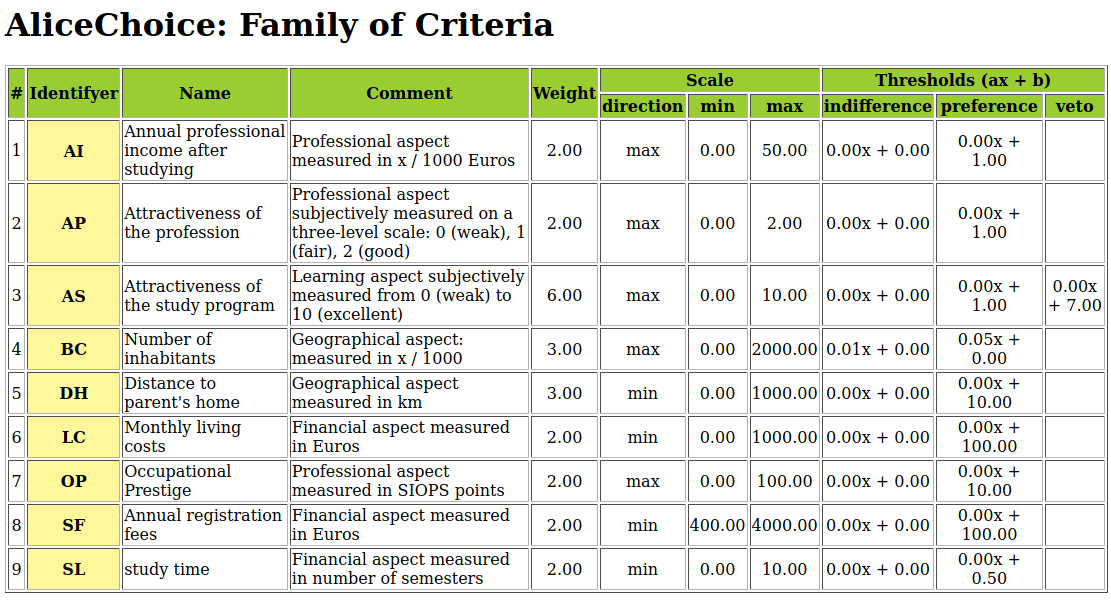
\includegraphics[width=\hsize]{Figures/12-2-aliceCriteria.png}
\caption{Alice's performance criteria}
\label{fig:12.2}       % Give a unique label
\end{figure}

It is worthwhile noticing in Figure~\vref{fig:12.2} that, on her subjective attractiveness scale of the study programs (criterion \texttt{AS}), Alice considers a performance differences of 7 points to be \emph{considerable} and triggering, the case given, an outranking polarisation \citep{BIS-2013}. Notice also the proportional \emph{indifference} ($1\%$) and \emph{preference} ($5\%$) discrimination thresholds shown on criterion \texttt{BC} (number of inhabitants).

Alice is subjectively evaluating the \emph{Attractiveness} of the studies (criterion \texttt{AS}) on an ordinal scale from \emph{weak} ($0$) to \emph{excellent} ($10$). Similarly, she is subjectively evaluating the \emph{Attractiveness} of the respective professions (criterion \texttt{AP}) on a three level ordinal scale from \emph{weak} ($0$), \emph{fair} ($1$) to \emph{good} ($2$). Considering the \emph{Occupational Prestige} (criterion \texttt{OP}), she looked up the SIOPS \footnote{Standard International Occupational Prestige Scale \citep*{GAN-1996}.}. All the other evaluation data she found on the internet.

In the \emph{heatmap view} shown in Figure~\vref{fig:12.3}, we may now consult Alice's performance evaluations.
\begin{lstlisting}
>>> t.showHTMLPerformanceHeatmap(\
...       colorLevels=5,Correlations=True,ndigits=0)
\end{lstlisting}
\begin{figure}[ht]
%\sidecaption
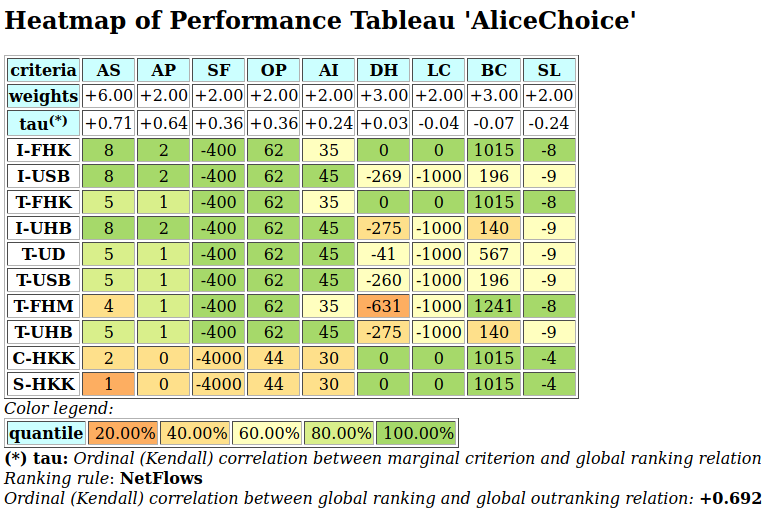
\includegraphics[width=\hsize]{Figures/12-3-aliceHeatmap.png}
\caption{Heatmap of Alice's performance tableau}
\label{fig:12.3}       % Give a unique label
\end{figure}

Her ten potential study programs are ordered with the \NetFlows ranking rule applied to the corresponding bipolar-valued outranking digraph (see Sec.~\ref{sec:8.3}). \emph{Graduate interpreter} studies in Köln (\texttt{I-FHK}) or Saarbrücken (\texttt{I-USB}), followed by \emph{Qualified Translator} studies in Köln (\texttt{T-FHK}) appear to be Alice's most preferred alternatives. The least attractive for her appear to be studies at the Chamber of Commerce of Köln (\texttt{C-HKK}, \texttt{S-HKK}). Notice by the way that evaluations on performance criteria to be \emph{minimised}, like \emph{Distance to Home} (criterion \texttt{DH}) or \emph{Study time} (criterion \texttt{SL}), are registered as \emph{negative} values, so that smaller measures are, in this case, preferred to larger ones.

It is finally interesting to observe in Figure~\vref{fig:12.3} (third row) that the \emph{most significant} performance criteria, appear to be for Alice, on the one side, the \emph{Attractiveness} of the study program (criterion \texttt{AS}, tau = $+0.72$) followed by the \emph{Attractiveness} of the future profession (criterion \texttt{AP}, tau = $+0.62$). On the other side, \emph{Study times} (criterion \texttt{SL}, tau = $-0.24$), \emph{Big city} (criterion \texttt{BC}, tau = $-0.07$) as well as \emph{Monthly living costs} (criterion \texttt{LC}, tau = $-0.04$) appear to be \emph{not so significant} (see Chap.~\ref{sec:16}).

\section{Building a best choice recommendation}
\label{sec:12.3}

Let us now have a look at the resulting pairwise outranking situations.
\begin{lstlisting}[caption={Computing Alice's outranking digraph},label=list:12.2]
>>> from outrankingDigraphs import BipolarOutrankingDigraph
>>> dg = BipolarOutrankingDigraph(t) 
>>> dg
  *------- Object instance description ------*
   Instance class      : BipolarOutrankingDigraph
   Instance name       : rel_AliceChoice
   Actions             : 10
   Criteria            : 9
   Size                : 67
   Determinateness (%) : 73.91
   Valuation domain    : [-1.00;1.00]
>>> dg.computeSymmetryDegree(Comments=True)
  Symmetry degree of graph <rel_AliceChoice> : 0.49
\end{lstlisting}

From Alice's performance tableau we obtain in the digraph \texttt{dg}  67 positively validated pairwise outranking situations, supported by a $74\%$ majority of criteria significance (see Lines 9-10 in List.~\vref{list:12.2}).

Due to the poorly discriminating performance evaluations, nearly half of these outranking situations (see Line 12) are \emph{symmetric} and reveal actually \emph{more or less indifference} situations between the potential study programs. This is well illustrated in the \emph{relation map} of the outranking digraph shown in Figure~\vref{fig:12.4}.
\begin{figure}[ht]
%\sidecaption
\includegraphics[width=10cm]{Figures/12-4-aliceRelationmap.png}
\caption{\Copeland ranked outranking relation map}
\label{fig:12.4}       % Give a unique label
\end{figure}
\begin{lstlisting}
>>> dg.showHTMLRelationMap(\
...           tableTitle='Outranking relation map',\
...           rankingRule='Copeland')
\end{lstlisting}

We have mentioned that Alice considers a performance difference of $7$ points on the \emph{Attractiveness of studies} criterion \texttt{AS} to be considerable which triggers, the case given, a potential polarisation of the outranking characteristics. In Figure~\vref{fig:12.4}, these polarisations appear in the last column and last row. The \texttt{showPolarisations()} method \index{showPolarisations@\texttt{showPolarisations()}} is useful for inspecting the occurrence of outranking polarisations.
\begin{lstlisting}[caption={Inspecting polarised outranking situations},label=list:12.3]
>>> dg.showPolarisations()
  *----  Negative polarisations ----*
   number of negative polarisations : 3 
    1: r(S-HKK >= I-FHK) = -0.17
     criterion: AS
     Considerable performance difference : -7.00
     Veto discrimination threshold       : -7.00
     Polarisation: r(S-HKK >= I-FHK) = -0.17 ==> -1.00
    2: r(S-HKK >= I-USB) = -0.17
     criterion: AS
     Considerable performance difference : -7.00
     Veto discrimination threshold       : -7.00
     Polarisation: r(S-HKK >= I-USB) = -0.17 ==> -1.00
    3: r(S-HKK >= I-UHB) = -0.17
     criterion: AS
     Considerable performance difference : -7.00
     Veto discrimination threshold       : -7.00
     Polarisation: r(S-HKK >= I-UHB) = -0.17 ==> -1.00
  *----  Positive polarisations ----*
   number of positive polarisations: 3 
    1: r(I-FHK >= S-HKK) = 0.83
     criterion: AS
     Considerable performance difference : 7.00
     Counter-veto threshold              : 7.00
     Polarisation: r(I-FHK >= S-HKK) = 0.83 ==> +1.00
    2: r(I-USB >= S-HKK) = 0.17
     criterion: AS
     Considerable performance difference : 7.00
     Counter-veto threshold              : 7.00
     Polarisation: r(I-USB >= S-HKK) = 0.17 ==> +1.00
    3: r(I-UHB >= S-HKK) = 0.17
     criterion: AS
     Considerable performance difference : 7.00
     Counter-veto threshold              : 7.00
     Polarisation: r(I-UHB >= S-HKK) = 0.17 ==> +1.00
\end{lstlisting}

In Listing~\vref{list:12.3}, we see that \emph{considerable} performance differences concerning the \emph{Attractiveness of the studies} (\texttt{AS} criterion) are indeed observed between the \emph{Specialised Secretary} study programm offered in Köln and the \emph{Graduate Interpreter} study programs offered in Köln, Saarbrücken and Heidelberg. They polarise, hence, three \emph{more or less invalid} outranking situations to \emph{certainly invalid} (Lines 8, 13, 18) and corresponding three \emph{more or less valid} converse outranking situations to \emph{certainly valid} ones (Lines 25, 30, 35). 

One may finally notice in the relation map, shown in Figure~\vref{fig:12.4}, that the four best-ranked study programs, \texttt{I-FHK}, \texttt{I-USB}, \texttt{I-UHB} and \texttt{T-FHK},  are in fact \Condorcet winners (see List.~\vref{list:12.4} Line 2), i.e. they are all four \emph{indifferent} one of the other \textbf{and} positively \emph{outranking} all other alternatives, a result confirmed in Listing~\vref{list:12.4} below by our \Rubis best choice recommendation (Chap.~\ref{sec:4} and \citealp*{BIS-2008a}).
\begin{lstlisting}[caption={Alice's best choice recommendation},label=list:12.4]
>>> dg.computeCondorcetWinners()
  ['I-FHK', 'I-UHB', 'I-USB', 'T-FHK'] 
>>> dg.showBestChoiceRecommendation()
  Best choice recommendation(s) (BCR)
    (in decreasing order of determinateness)   
    Credibility domain: [-1.00,1.00]
   === >> potential first choice(s)
   choice                : ['I-FHK','I-UHB','I-USB','T-FHK']
     independence        : 0.17
     dominance           : 0.08
     absorbency          : -0.83
     covering (%)        : 62.50
     determinateness (%) : 68.75
     most credible action(s) = {'I-FHK': 0.75,'T-FHK': 0.17,
                                'I-USB': 0.17,'I-UHB': 0.17}
   === >> potential last choice(s) 
   choice                : ['C-HKK', 'S-HKK']
     independence        : 0.50
     dominance           : -0.83
     absorbency          : 0.17
     covered (%)         : 100.00
     determinateness (%) : 58.33
     most credible action(s) = {'S-HKK': 0.17,'C-HKK': 0.17}
\end{lstlisting}

Most credible best choice among the four best-ranked study programs eventually becomes the \emph{Graduate Interpreter} study program at the Technical High School in Köln (see Line 14) supported by a $(0.75 + 1)/2.0 \,=\,87.5\% (18/24)$ majority of global criteria significance \footnote{See Sec.~\ref{sec:4.5} on computing best choice recommendations and Sec.~\ref{sec:17.6} on solving kernel equation systems.}

In the relation map, shown in Figure~\vref{fig:12.4}, we see in the left lower corner that the \emph{asymmetric part} of the outranking relation, i.e. the corresponding \emph{strict} outranking relation, is actually \emph{transitive} (see Line 3 in List.~\vref{list:12.5} below). Hence, a \emph{graphviz} drawing of its \emph{skeleton}, oriented by the previous \emph{first}, respectively \emph{last} choice, may well illustrate our \emph{best choice recommendation}. The \texttt{Reverse=True} flag in Line 4 eliminates the transitivity induced arcs from digraph \texttt{dgcd}.\index{closeTransitive@\texttt{closeTransitive()}}
\begin{lstlisting}[caption={Alice's strict best choice recommendation},label=list:12.5]
>>> dgcd = ~(-dg)
>>> dgcd.isTransitive()
    True
>>> dgcd.closeTransitive(Reverse=True,InSite=True)
>>> dgcd.exportGraphViz('aliceBestChoice',\
...                     firstChoice=['I-FHK'],\
...                     lastChoice=['S-HKK','C-HKK'])
  *---- exporting a dot file for GraphViz tools ---------*
   Exporting to aliceBestChoice.dot
   dot -Grankdir=BT -Tpng aliceBestChoice.dot -o aliceBestChoice.png
\end{lstlisting}
\begin{figure}[ht]
\sidecaption[t]
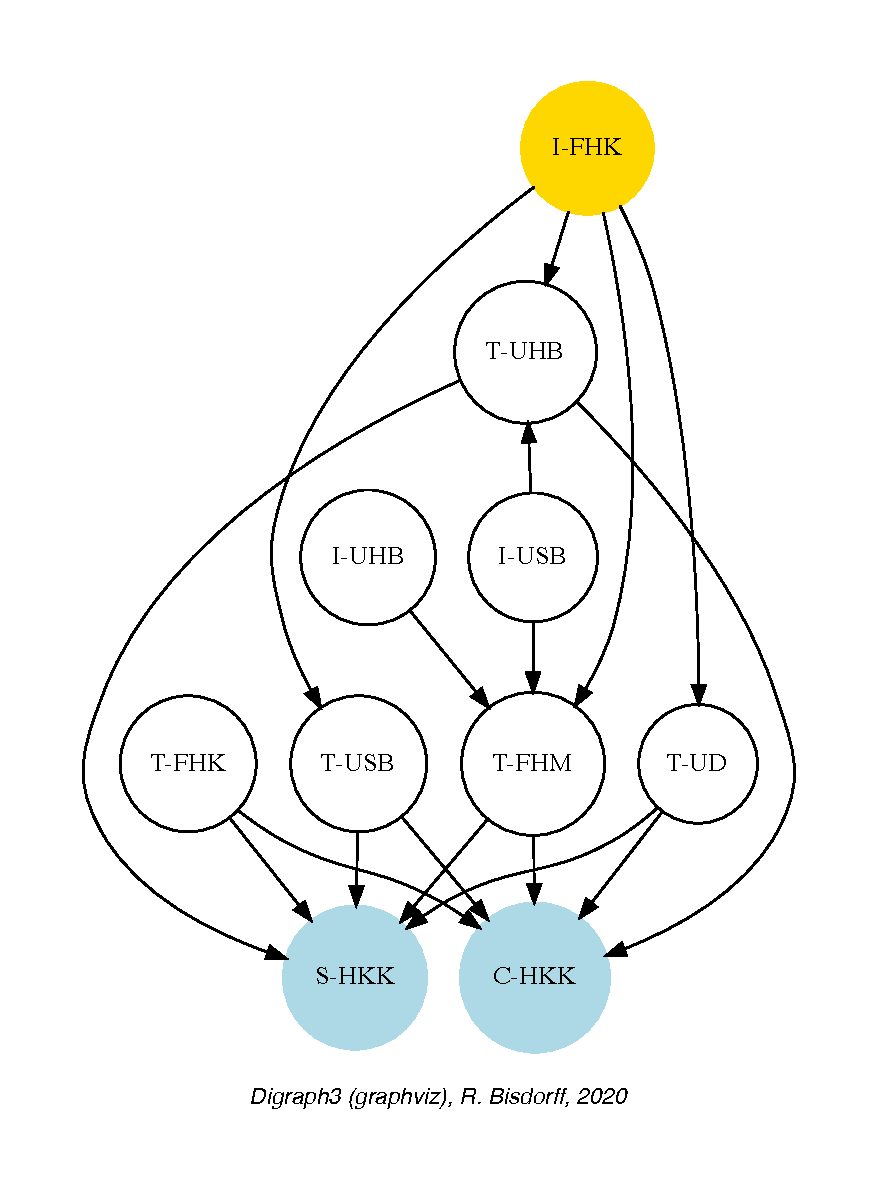
\includegraphics[width=7cm]{Figures/12-5-aliceBestChoice.pdf}
\caption[Alice's best choice recommendation]{\emph{Alice's best choice recommendation}. We notice that the \emph{Graduate Interpreter} studies come first, followed by the \emph{Qualified Translator} studies. Last come the \emph{Chamber of Commerce}'s specialised studies. This confirms again the high significance that Alice attaches to the \emph{attractiveness} of her further studies and of her future profession (see criteria \texttt{AS} and \texttt{AP} in Fig.~\vref{fig:12.3})}
\label{fig:12.5}       % Give a unique label
\end{figure}

Let us now, for instance, check the pairwise outranking situations observed between the first and second-ranked alternative, i.e. \emph{Graduate Interpreter} studies in Köln versus \emph{Graduate Interpreter} studies in Saarbrücken (see \texttt{I-FHK} and \texttt{I-USB} in Fig.~\vref{fig:12.3}).\index{showHTMLPairwiseOutrankings@\texttt{showHTMLPairwiseOutrankings()}}
\begin{lstlisting}
>>> dg.showHTMLPairwiseOutrankings('I-FHK','I-USB')
\end{lstlisting}
\begin{figure}[ht]
\sidecaption[t]
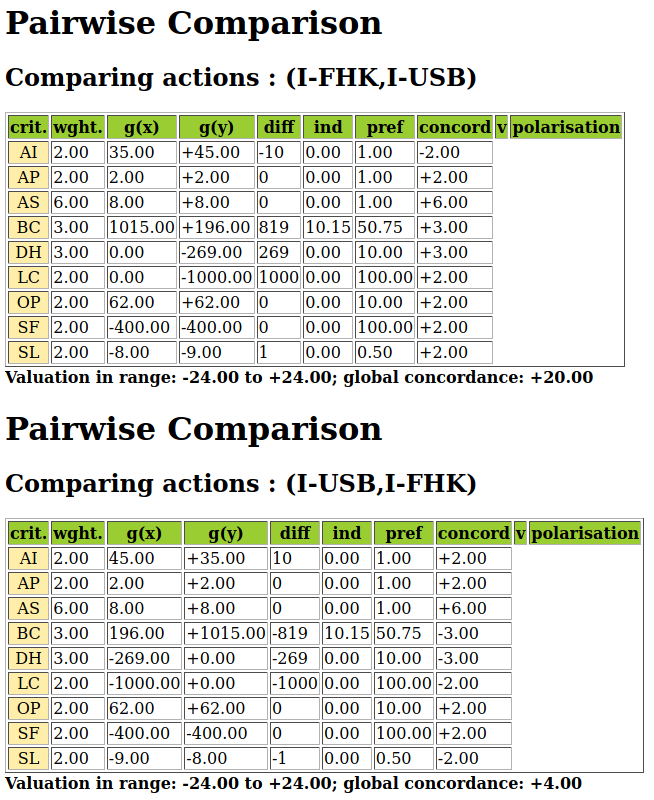
\includegraphics[width=7cm]{Figures/12-6-pairwiseComparison.png}
\caption[Comparing the first and second best-ranked study programs]{\emph{Comparing the first and second best-ranked study programs}. The Köln alternative is \emph{at least as well evaluated as} the Saarbrücken alternative on all the performance criteria, except the \emph{Annual income} (of significance $2/24$). Conversely, the Saarbrücken alternative is clearly \emph{outperformed} from the geographical ($0/6$) as well as from the financial perspective ($2/6$)}
\label{fig:12.6}       % Give a unique label
\end{figure}
%\clearpage

In a similar way, one may finally compute a \emph{weak ranking} of all the potential study programs with the help of the \texttt{RankingByChoosingDigraph} class\index{RankingByChoosingDigraph@\texttt{RankingByChoosingDigraph} class} from the \texttt{transitiveDigraphs} module\index{transitiveDigraphs@\texttt{transitiveDigraphs} module}, that computes a bipolar ranking by conjointly \emph{best-choosing} and \emph{last-rejecting} \citep{BIS-1999}.
\begin{lstlisting}[caption={Weakly ranking by bipolar best-choosing and last-rejecting},label=list:12.6]
>>> from transitiveDigraphs import\
...               RankingByChoosingDigraph
>>> rbc = RankingByChoosingDigraph(dg)
>>> rbc.showRankingByChoosing()
    Ranking by Choosing and Rejecting
     1st ranked ['I-FHK'] 
       2nd ranked ['I-USB']
	 3rd ranked ['I-UHB']
	   4th ranked ['T-FHK']
	     5th ranked ['T-UD']
	     5th last ranked ['T-UD']
	   4th last ranked ['T-UHB', 'T-USB']
	 3rd last ranked ['T-FHM']
       2nd last ranked ['C-HKK']
     1st last ranked ['S-HKK']
\end{lstlisting}

In Listing~\vref{list:12.6}, we find confirmed that the \emph{Interpreter} studies appear all preferred to the \emph{Translator} studies. Furthermore, the \emph{Interpreter} studies in Saarbrücken appear preferred to the same studies in Heidelberg. The Köln alternative is apparently the preferred one of all the \emph{Translater} studies. And, the \emph{Foreign Correspondent} and the \emph{Specialised Secretary} studies appear second-last and last ranked.

Yet, how \emph{robust} are our findings with respect to potential settings of the decision objectives' importance and the performance criteria significance weights?
		
\section{Robustness analysis}
\label{sec:12.4}

Alice considers her four decision objectives as being \emph{more or less} equally important. Here we have, however, allocated \emph{strictly equal} importance weights with \emph{strictly equi-significant} criteria per objective. How robust is the previous best choice recommendation when, now, we would consider the importance of the objectives and, hence, the significance of the respective performance criteria to be \emph{more or less uncertain}?

To answer this question, we consider the respective criteria significance weights $w_j$ for $j=1,...,9$ to be \emph{triangular random variables} in the range 0 to $2w_j$ with mode = $w_j$. Computing a corresponding $90\%$-\emph{confident} outranking digraph may be done with the help of the \texttt{ConfidentBipolarOutrankingDigraph} class\index{ConfidentBipolarOutrankingDigraph@\texttt{ConfidentBipolarOutranking\-Digraph} class} (see Chap.~\ref{sec:18}).
\begin{lstlisting}[caption={Computing the 90\% confident outranking digraph},label=list:12.7]
>>> from outrankingDigraphs import\
...         ConfidentBipolarOutrankingDigraph
>>> cdg = ConfidentBipolarOutrankingDigraph(t,\
...         distribution='triangular',confidence=90.0)
>>> cdg
  *------- Object instance description ------*
    Instance class       : ConfidentBipolarOutrankingDigraph
    Instance name        : rel_AliceChoice_CLT
    Actions              : 10
    Criteria             : 9
    Size                 : 44
    Valuation domain     : [-1.00;1.00]
    Uncertainty model    : triangular(a=0,b=2w) 
    Likelihood domain    : [-1.0;+1.0] 
    Confidence level     : 90.0% 
    Confident majority   : 14/24 (58.3%) 
    Determinateness (%)  : 68.19
\end{lstlisting}

Of the original 67 valid outranking situations, 44 outranking situations are retained as being $90\%$-confident (see List.~\vref{list:12.7} Line 11). The corresponding $90\%$-confident \emph{qualified majority} of criteria significance amounts to $14/24 = 58.3\%$ (Line 16).  

Concerning now a $90\%$-confident best choice recommendation, we are lucky. 
\begin{lstlisting}[caption={Computing the $90\%$-confident best choice recommendation.},label=list:12.8]
>>> cdg.computeCondorcetWinners()
  ['I-FHK']
>>> cdg.showBestChoiceRecommendation()
  ***********************
  Best choice recommendation(s) (BCR)
   (in decreasing order of determinateness)   
   Credibility domain: [-1.00,1.00]
  === >> potential best choice(s)
   choice              : ['I-FHK','I-UHB','I-USB',
                          'T-FHK','T-FHM']
      independence        : 0.00
      dominance           : 0.42
      absorbency          : 0.00
      covering (%)        : 20.00
      determinateness (%) : 61.25
   - most credible action(s) = { 'I-FHK': 0.75, }
\end{lstlisting}

The \emph{Graduate Interpreter} studies in Köln remain indeed a 90\%-confident \Condorcet winner (see Fig.~\vref{fig:12.7} Line 2). Hence, the same study program also remains our 90\%-confident most credible best choice supported by a comfortable $18/24 (87.5\%)$ majority of the global criteria significance (see Lines 9-10 and 16 in List.~\vref{list:12.8}).

When previously comparing the two best-ranked study programs (see Fig.~\vref{fig:12.6}), we have observed that \texttt{I-FHK} actually positively outranks \texttt{I-USB} on all four decision objectives. When admitting equi-significant criteria significances per objective, this outranking situation is hence valid independently of the importance weights Alice may allocate to each of her decision objectives. 

The \texttt{UnOpposedBipolarOutrankingDigraph} class\index{UnOpposedBipolarOutrankingDigraph@\texttt{UnOpposedBipolarOutrankingDigraph} class} constructor from the \texttt{outrankingDigraphs} module computes these \emph{unopposed} outranking situations (see Sec.~\ref{sec:19.5}).
\begin{lstlisting}[caption={Computing the unopposed outranking situations},label=list:12.9]
>>> from outrankingDigraphs import\
...                     UnOpposedBipolarOutrankingDigraph
>>> uop = UnOpposedBipolarOutrankingDigraph(t)
>>> uop
  *------- Object instance description ------*
   Instance class       : UnOpposedBipolarOutrankingDigraph
   Instance name        : AliceChoice_unopposed_outrankings
   Actions              : 10
   Criteria             : 9
   Size                 : 28
   Oppositeness (%)     : 58.21
   Determinateness (%)  : 62.94
   Valuation domain     : [-1.00;1.00]
>>> uop.isTransitive()
  True
\end{lstlisting}

28 out the 67 standard outranking situations remain valid, which leads to an \emph{oppositeness degree}\index{oppositeness degree} of $(1.0 - 28/67) = 58.21\%$ (see Lines 10-11 in List.~\vref{list:12.9}). Remarkable furthermore is that this unopposed outranking digraph \texttt{uop} is actually \emph{transitive}, i.e. modelling a \emph{partial ranking} of the study programs (Lines 14-15).

The \texttt{exportGraphViz()} method of the \texttt{Transi\-tiveDigraph} class\index{TransitiveDigraph@\texttt{TransitiveDigraph} class} draws the corresponding partial ranking.
\begin{lstlisting}
>>> from transitiveDigraphs import TransitiveDigraph
>>> TransitiveDigraph.exportGraphViz(uop,\
...           fileName='choiceUnopposed')
  *---- exporting a dot file for GraphViz tools ---------*
   Exporting to choiceUnopposed.dot
   dot -Grankdir=TB -Tpng choiceUnopposed.dot -o choiceUnopposed.png
\end{lstlisting}
\begin{figure}[ht]
\sidecaption[t]
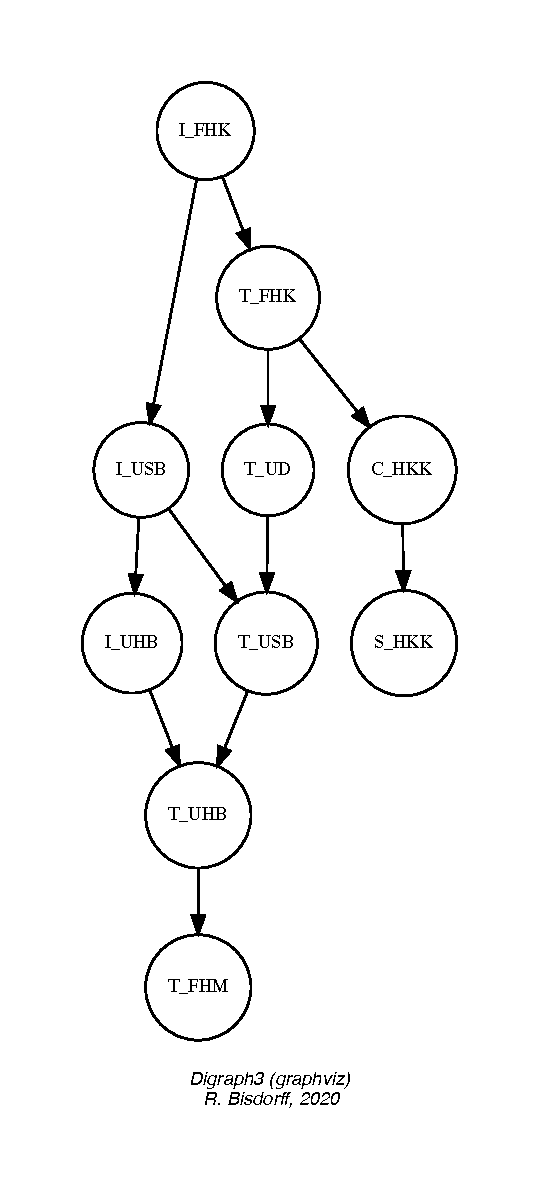
\includegraphics[width=6cm]{Figures/12-7-choiceUnopposed.pdf}
\caption[Unopposed partial ranking of the potential study programs]{\emph{Unopposed partial ranking of the potential study programs}. Again, when \emph{equally significant} performance criteria are assumed per decision objective, we observe in the Figure here that $I-FHK$ remains the stable best choice, \emph{independently} of the actual importance weights that Alice may wish to allocate to her four decision objectives}
\label{fig:12.7}       % Give a unique label
\end{figure}
%\clearpage

In view of her performance tableau shown in Figure~\vref{fig:12.3}, \emph{Graduate Interpreter} studies at the Technical High School Köln, thus, represent definitely \textbf{Alice's very best choice}.

%\vspace{1cm}
\vspace{\baselineskip}
For further reading about the \Rubis \emph{Best Choice} methodology, one may consult in \citet{BIS-2015bestPoster} the study of a \emph{real decision-aiding case} about choosing a best poster in a scientific conference.
 
%%%%%%% The chapter bibliography
%\normallatexbib
%\clearpage
%\phantomsection
%\addcontentsline{toc}{section}{Chapter Bibliography}
%\chapter{Alice's best choice: A selection case study}
\label{sec:12}
\abstract*{ The chapter presents a case study concerning the building of a best choice recommendation for Alice, a German student who wants some advice concerning the choice of her future University studies. We present Alice's performance tableau --potential foreign language study programs, her decision objectives, performance criteria and performance grades-- and build a best choice recommendation for her. A thorough robustness analysis confirms a very best choice.}

\abstract{ The chapter presents a case study concerning the building of a best choice recommendation for Alice, a German student who wants some advice concerning the choice of her future University studies. We present Alice's performance tableau --potential foreign language study programs, her decision objectives, performance criteria and performance grades-- and build a best choice recommendation for her. A thorough robustness analysis confirms a very best choice.}


\begin{figure}[ht]
\sidecaption

\includegraphics[width=4cm]{Figures/12-1-AliceF.png}
\caption{Alice D., 19 years old German student finishing her secondary studies in Köln (Germany), desires to undertake foreign languages studies.}
\label{fig:12.1}       % Give a unique label
\end{figure}

\noindent This case study is inspired by a multiple criteria decision analysis case study published by \citealp[pp. 1-17]{EIS-2001}.

\section{The decision problem}
\label{sec:12.1}

Alice will probably receive her "Abitur" with satisfactory and/or good marks and  wants to start her further studies thereafter. She would not mind staying in Köln, yet is ready to move elsewhere if necessary. The length of the higher studies do concern her, as she wants to earn her life as soon as possible.  Her parents however agree to financially support her study fees as well as her living costs during her studies.

Alice has already identified 10 potential study programs.
\begin{table}[h]
\caption{The potential study programs}
\label{tab:12.1}       % Give a unique label
\begin{center}
  %\begin{small}
    \begin{tabular}{l|l|l|l}
      \svhline\noalign{\smallskip}
      ID & Diploma & Institution & City\\
      \noalign{\smallskip}\hline\noalign{\smallskip}
      \texttt{T-UD}   & Qualified translator (T)  &   University (UD)               &  Düsseldorf\\
      \texttt{T-FHK}  & Qualified translator (T)  &   Higher Technical School (FHK) &  Köln\\
      \texttt{T-FHM}  & Qualified translator (T)  &   Higher Technical School (FHM) &  München\\
      \texttt{I-FHK}  & Graduate interpreter (I)  &   Higher Technical School (FHK) &  Köln\\
      \texttt{T-USB}  & Qualified translator (T)  &   University (USB)              &  Saarbrücken\\
      \texttt{I-USB}  & Graduate interpreter (I)  &   University (USB)              &  Saarbrücken\\
      \texttt{T-UHB}  & Qualified translator (T)  &   University (UHB)              &  Heidelberg\\
      \texttt{I-UHB}  & Graduate interpreter (I)  &   University (UHB)              &  Heidelberg\\
      \texttt{S-HKK}  & Specialized secretary (S) &   Chamber of Commerce (HKK)     &  Köln\\
      \texttt{C-HKK}  & Foreign correspondent (C) &   Chamber of Commerce (HKK)     &  Köln\\
      \noalign{\smallskip}\hline
    \end{tabular}
  %\end{small}
\end{center}
\end{table}

In Table~\vref{tab:12.1} we notice that Alice considers three \emph{Graduate Interpreter} studies (8 or 9 Semesters), respectively in Köln, in Saarbrücken or in Heidelberg; and five \emph{Qualified translator} studies (8 or 9 Semesters), respectively in Köln, in Düsseldorf, in Saarbrücken, in Heidelberg or in Munich. She also considers two short (4 Semesters) study programs at the Chamber of Commerce in Köln. 

Four \textbf{decision objectives} of more or less equal importance are guiding Alice's choice:
\begin{enumerate}[leftmargin=1cm,topsep=1pt]
\item \emph{maximize} the attractiveness of the study place (\texttt{GEO}),
\item \emph{maximize} the attractiveness of her further studies (\texttt{LEA}),
\item \emph{minimize}  her financial dependency on her parents (\texttt{FIN}),
\item \emph{maximize} her professional perspectives (\texttt{PRA}).
\end{enumerate}

The decision consequences Alice wishes to take into account for evaluating the potential study programs with respect to each of the four objectives are modelled by the following \emph{coherent family of criteria} \citep*{ROY-1991,ROY-1993}. Such a family of performance criteria verifies:
\begin{enumerate}[topsep=1pt]
\item \emph{Exhaustiveness}: No argument acceptable to Alice can be put forward to justify a preference in favour of study program $x$ versus program $y$  when $x$ and $y$ have the same performance level on each of the performance criteria;
\item \emph{Cohesiveness}: Alice recognizes that program $x$ must be preferred to program $y$ whenever the performance level of $x$ is significantly better than that of $y$ on one of the criteria of positive weight, performance levels of $x$ and $y$ being the same on each of the other criteria; 
\item \emph{Nonredundancy}: One of the above requirements is violated if one of the performance criteria is left out from the family.
\end{enumerate}

\begin{table}[h]
\caption{Alice's family of performance criteria}
\label{tab:12.2}       % Give a unique label
\begin{center}
  %\begin{small}
    \begin{tabular}{l|l|l|l|c}
      \svhline\noalign{\smallskip}
      ID & Name & Comment & Objective & Weight\\
      \noalign{\smallskip}\hline\noalign{\smallskip}
       \texttt{DH}  & Proximity  &  Distance in km to her home (min)      &   \texttt{GEO}    &     3\\
       \texttt{BC}  & Big City   &  Number of inhabitants (max)           &   \texttt{GEO}    &     3\\
       \   & \          &  \                                     &   \      &     \ \\
       \texttt{AS}  & Studies    &  Attractiveness of the studies (max)   &   \texttt{LEA}    &     6\\
       \   & \          &  \                                     &  \       &    \ \\
       \texttt{SF}  & Fees       &  Annual study fees (min)               &   \texttt{FIN}    &     2\\
       \texttt{LC}  & Living     &  Monthly living costs (min)            &   \texttt{FIN}    &     2\\
       \texttt{SL}  & Length     &  Length of the studies (min)           &   \texttt{FIN}    &     2\\
       \   &  \         &   \                                    &   \      &     \ \\
       \texttt{AP}  & Profession &  Attractiveness of the profession (max)&   \texttt{PRA}    &     2\\
       \texttt{AI}  & Income     &  Annual income after studying (max)    &   \texttt{PRA}    &     2\\
       \texttt{PR}  & Prestige   &  Occupational prestige (max)           &   \texttt{PRA}    &     2\\
      \noalign{\smallskip}\hline
    \end{tabular}
  %\end{small}
\end{center}
\end{table}

Within each decision objective, the performance criteria are considered to be \emph{equisignificant}. Hence, the four decision objectives get a same \emph{importance weight} of $6$ (see Table~\vref{tab:12.2} Column 5).

\section{The performance tableau}
\label{sec:12.2}

The actual evaluations of Alice's potential study programs are stored in a file named \texttt{AliceChoice.py} of \texttt{PerformanceTableau} format \footnote{The performance tableau \texttt{AliceChoice.py} may be found in the \texttt{examples} directory of the \Digraph resources\citep{BIS-2021}.}.
\begin{lstlisting}[caption={Alice's performance tableau},label=list:12.1]
>>> from perfTabs import PerformanceTableau
>>> t = PerformanceTableau('AliceChoice')
>>> t.showObjectives()
  *------ decision objectives -------"
    GEO: Geographical aspect
     DH Distance to parent's home 3
     BC Number of inhabitants     3
     Total weight: 6 (2 criteria)
    LEA: Learning aspect
     AS Attractiveness of the study program 6
     Total weight: 6.00 (1 criteria)
    FIN: Financial aspect
     SF Annual registration fees 2
     LC Monthly living costs     2
     SL Study time               2
     Total weight: 6.00 (3 criteria)
    PRA: Professional aspect
     AP Attractiveness of the profession          2
     AI Annual professional income after studying 2
     OP Occupational Prestige                     2
     Total weight: 6.00 (3 criteria)
\end{lstlisting}

Details of the performance criteria may be consulted in the browser view below.\index{showHTMCriteria@\texttt{showHTMCriteria()}}
\begin{lstlisting}
>>> t.showHTMLCriteria()
\end{lstlisting}
\begin{figure}[ht]
%\sidecaption
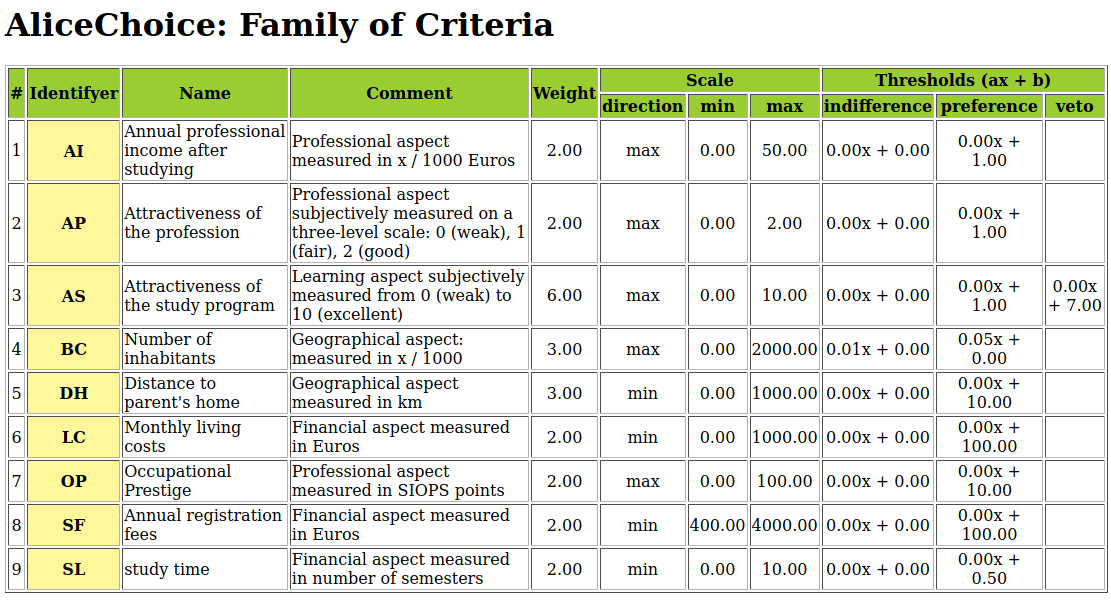
\includegraphics[width=\hsize]{Figures/12-2-aliceCriteria.png}
\caption{Alice's performance criteria}
\label{fig:12.2}       % Give a unique label
\end{figure}

It is worthwhile noticing in Fig.~\vref{fig:12.2} that, on her subjective attractiveness scale of the study programs (criterion \texttt{AS}), Alice considers a performance differences of 7 points to be \emph{considerable} and triggering, the case given, an outranking polarisation \citep{BIS-2013}. Notice also the proportional \emph{indifference} ($1\%$) and \emph{preference} ($5\%$) discrimination thresholds shown on criterion \texttt{BC} (number of inhabitants).

Alice is subjectively evaluating the \emph{Attractiveness} of the studies (criterion \texttt{AS}) on an ordinal scale from \emph{weak} ($0$) to \emph{excellent} ($10$). Similarly, she is subjectively evaluating the \emph{Attractiveness} of the respective professions (criterion \texttt{AP}) on a three level ordinal scale from \emph{weak} ($0$), \emph{fair} ($1$) to \emph{good} ($2$). Considering the \emph{Occupational Prestige} (criterion \texttt{OP}), she looked up the SIOPS \footnote{Standard International Occupational Prestige Scale \citep*{GAN-1996}.}. All the other evaluation data she found on the internet.

In the \emph{heatmap view} shown in Fig.~\vref{fig:12.3}, we may now consult Alice's performance gradings.
\begin{lstlisting}
>>> t.showHTMLPerformanceHeatmap(\
...       colorLevels=5,Correlations=True,ndigits=0)
\end{lstlisting}
\begin{figure}[ht]
%\sidecaption
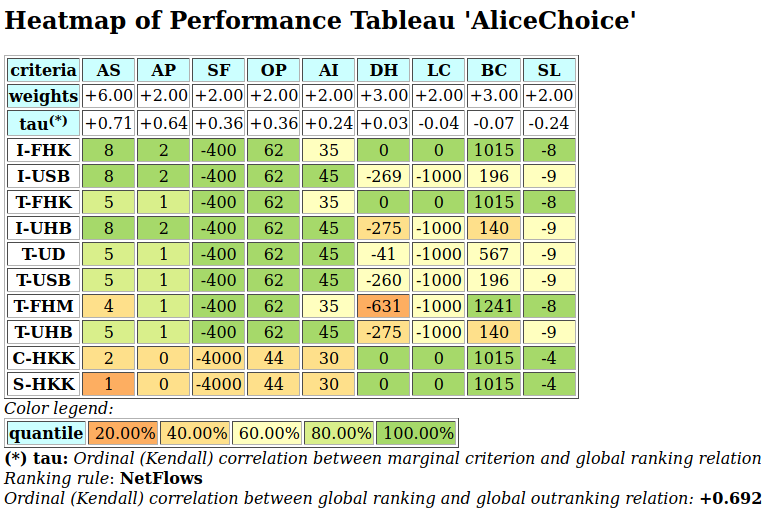
\includegraphics[width=\hsize]{Figures/12-3-aliceHeatmap.png}
\caption{Heatmap of Alice's performance tableau}
\label{fig:12.3}       % Give a unique label
\end{figure}

Her ten potential study programs are ordered with the \NetFlows ranking rule applied to the corresponding bipolar-valued outranking digraph (see Section~\vref{sec:8.3}). \emph{Graduate interpreter} studies in Köln (\texttt{I-FHK}) or Saarbrücken (\texttt{I-USB}), followed by \emph{Qualified Translator} studies in Köln (\texttt{T-FHK}) appear to be Alice's most preferred alternatives. The least attractive for her appear to be studies at the Chamber of Commerce of Köln (\texttt{C-HKK}, \texttt{S-HKK}). Notice by the way that evaluations on performance criteria to be \emph{minimized}, like \emph{Distance to Home} (criterion \texttt{DH}) or \emph{Study time} (criterion \texttt{SL}), are registered as \emph{negative} values, so that smaller measures are, in this case, preferred to larger ones.

It is finally interesting to observe in Fig.~\vref{fig:12.3} (third row) that the \emph{most significant} performance criteria, appear to be for Alice, on the one side, the \emph{Attractiveness} of the study program (criterion \texttt{AS}, tau = $+0.72$) followed by the \emph{Attractiveness} of the future profession (criterion \texttt{AP}, tau = $+0.62$). On the other side, \emph{Study times} (criterion \texttt{SL}, tau = $-0.24$), \emph{Big city} (criterion \texttt{BC}, tau = $-0.07$) as well as \emph{Monthly living costs} (criterion \texttt{LC}, tau = $-0.04$) appear to be \emph{not so significant} (see Chapter~\vref{sec:16}).

\section{Building a best choice recommendation}
\label{sec:12.3}

Let us now have a look at the resulting pairwise outranking situations.
\begin{lstlisting}[caption={Computing Alice's outranking digraph},label=list:12.2]
>>> from outrankingDigraphs import BipolarOutrankingDigraph
>>> dg = BipolarOutrankingDigraph(t) 
>>> dg
  *------- Object instance description ------*
   Instance class      : BipolarOutrankingDigraph
   Instance name       : rel_AliceChoice
   Actions             : 10
   Criteria            : 9
   Size                : 67
   Determinateness (%) : 73.91
   Valuation domain    : [-1.00;1.00]
>>> dg.computeSymmetryDegree(Comments=True)
  Symmetry degree of graph <rel_AliceChoice> : 0.49
\end{lstlisting}

From Alice's performance tableau we obtain in the digraph \texttt{dg}  67 positively validated pairwise outranking situations, supported by a $74\%$ majority of criteria significance (see Lines 9-10 in Listing~\vref{list:12.2}).

Due to the poorly discriminating performance evaluations, nearly half of these outranking situations (see Line 12) are \emph{symmetric} and reveal actually \emph{more or less indifference} situations between the potential study programs. This is well illustrated in the \emph{relation map} of the outranking digraph shown in Fig.~\vref{fig:12.4}.
\begin{figure}[ht]
%\sidecaption
\includegraphics[width=10cm]{Figures/12-4-aliceRelationmap.png}
\caption{\Copeland ranked outranking relation map}
\label{fig:12.4}       % Give a unique label
\end{figure}
\begin{lstlisting}
>>> dg.showHTMLRelationMap(\
...           tableTitle='Outranking relation map',\
...           rankingRule='Copeland')
\end{lstlisting}

We have mentioned that Alice considers a performance difference of $7$ points on the \emph{Attractiveness of studies} criterion \texttt{AS} to be considerable which triggers, the case given, a potential polarisation of the outranking characteristics. In Fig.~\vref{fig:12.4}, these polarisations appear in the last column and last row. We may inspect the occurrence of such polarisations with the \texttt{showPolarisations()} method. \index{showPolarisations@\texttt{showPolarisations()}}
\begin{lstlisting}[caption={Polarised outranking situations},label=list:12.3]
>>> dg.showPolarisations()
  *----  Negative polarisations ----*
   number of negative polarisations : 3 
    1: r(S-HKK >= I-FHK) = -0.17
     criterion: AS
     Considerable performance difference : -7.00
     Veto discrimination threshold       : -7.00
     Polarisation: r(S-HKK >= I-FHK) = -0.17 ==> -1.00
    2: r(S-HKK >= I-USB) = -0.17
     criterion: AS
     Considerable performance difference : -7.00
     Veto discrimination threshold       : -7.00
     Polarisation: r(S-HKK >= I-USB) = -0.17 ==> -1.00
    3: r(S-HKK >= I-UHB) = -0.17
     criterion: AS
     Considerable performance difference : -7.00
     Veto discrimination threshold       : -7.00
     Polarisation: r(S-HKK >= I-UHB) = -0.17 ==> -1.00
  *----  Positive polarisations ----*
   number of positive polarisations: 3 
    1: r(I-FHK >= S-HKK) = 0.83
     criterion: AS
     Considerable performance difference : 7.00
     Counter-veto threshold              : 7.00
     Polarisation: r(I-FHK >= S-HKK) = 0.83 ==> +1.00
    2: r(I-USB >= S-HKK) = 0.17
     criterion: AS
     Considerable performance difference : 7.00
     Counter-veto threshold              : 7.00
     Polarisation: r(I-USB >= S-HKK) = 0.17 ==> +1.00
    3: r(I-UHB >= S-HKK) = 0.17
     criterion: AS
     Considerable performance difference : 7.00
     Counter-veto threshold              : 7.00
     Polarisation: r(I-UHB >= S-HKK) = 0.17 ==> +1.00
\end{lstlisting}

In Listing~\vref{list:12.3}, we see that \emph{considerable} performance differences concerning the \emph{Attractiveness of the studies} (\texttt{AS} criterion) are indeed observed between the \emph{Specialised Secretary} study programm offered in Köln and the \emph{Graduate Interpreter} study programs offered in Köln, Saarbrücken and Heidelberg. They polarise, hence, three \emph{more or less invalid} outranking situations to \emph{certainly invalid} (Lines 8, 13, 18) and corresponding three \emph{more or less valid} converse outranking situations to \emph{certainly valid} ones (Lines 25, 30, 35). 

We may finally notice in the relation map, shown in Fig.~\vref{fig:12.4}, that the four best-ranked study programs, \texttt{I-FHK}, \texttt{I-USB}, \texttt{I-UHB} and \texttt{T-FHK},  are in fact \Condorcet winners (see Listing~\vref{list:12.4} Line 2), i.e. they are all four \emph{indifferent} one of the other \textbf{and} positively \emph{outranking} all other alternatives, a result confirmed in Listing~\vref{list:12.4} below by our \Rubis best choice recommendation \citep*{BIS-2008a}.
\begin{lstlisting}[caption={Alice's best choice recommendation},label=list:12.4]
>>> dg.computeCondorcetWinners()
  ['I-FHK', 'I-UHB', 'I-USB', 'T-FHK'] 
>>> dg.showBestChoiceRecommendation()
  Best choice recommendation(s) (BCR)
    (in decreasing order of determinateness)   
    Credibility domain: [-1.00,1.00]
   === >> potential best choice(s)
   choice                : ['I-FHK','I-UHB','I-USB','T-FHK']
     independence        : 0.17
     dominance           : 0.08
     absorbency          : -0.83
     covering (%)        : 62.50
     determinateness (%) : 68.75
     most credible action(s) = {'I-FHK': 0.75,'T-FHK': 0.17,
                                'I-USB': 0.17,'I-UHB': 0.17}
   === >> potential worst choice(s) 
   choice                : ['C-HKK', 'S-HKK']
     independence        : 0.50
     dominance           : -0.83
     absorbency          : 0.17
     covered (%)         : 100.00
     determinateness (%) : 58.33
     most credible action(s) = {'S-HKK': 0.17,'C-HKK': 0.17}
\end{lstlisting}

Most credible best choice among the four best-ranked study programs eventually becomes the \emph{Graduate Interpreter} study program at the Technical High School in Köln (see Line 14) supported by a $(0.75 + 1)/2.0 \,=\,87.5\% (18/24)$ majority of global criteria significance \footnote{See Section~\vref{sec:17.6} on solving \Berge kernel equation systems.}.

In the relation map, shown in Fig.~\vref{fig:12.4}, we see in the left lower corner that the \emph{asymmetric part} of the outranking relation, i.e. the corresponding \emph{strict} outranking relation, is actually \emph{transitive} (see Line 2 below). Hence, a \emph{graphviz} drawing of its \emph{skeleton}, oriented by the previous \emph{best}, respectively \emph{worst} choice, may well illustrate our \emph{best choice recommendation}.
\begin{lstlisting}[caption={Alice's strict best choice recommendation},label=list:12.5]
>>> dgcd = ~(-dg)
>>> dgcd.isTransitive()
    True
>>> dgcd.closeTransitive(Reverse=True,InSite=True)
>>> dgcd.exportGraphViz('aliceBestChoice',\
...                     bestChoice=['I-FHK'],\
...                     worstChoice=['S-HKK','C-HKK'])
  *---- exporting a dot file for GraphViz tools ---------*
   Exporting to aliceBestChoice.dot
   dot -Grankdir=BT -Tpng aliceBestChoice.dot -o aliceBestChoice.png
\end{lstlisting}
\begin{figure}[ht]
\sidecaption[t]
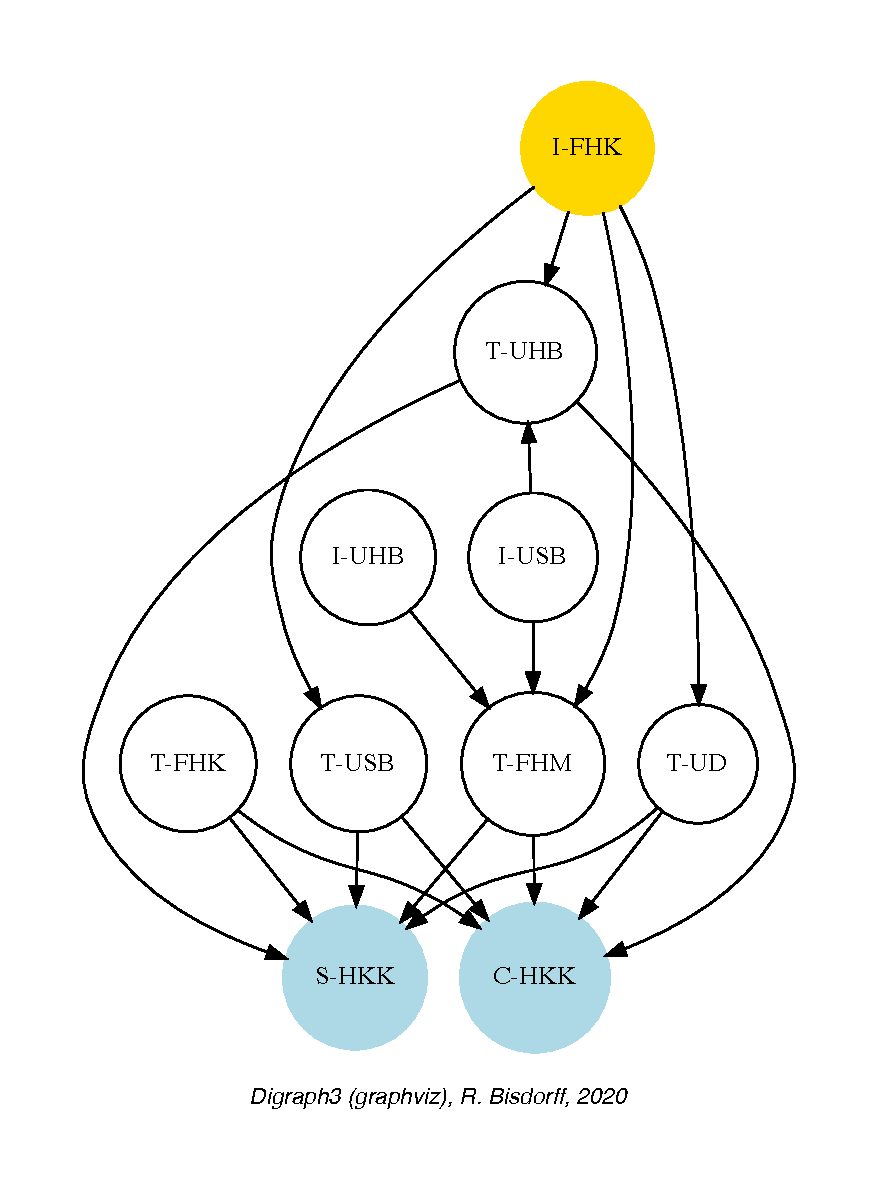
\includegraphics[width=7cm]{Figures/12-5-aliceBestChoice.pdf}
\caption{In Alice's best choice recommendation, we notice that the \emph{Graduate Interpreter} studies come first, followed by the \emph{Qualified Translator} studies. Last come the \emph{Chamber of Commerce}'s specialised studies. This confirms again the high significance that Alice attaches to the \emph{attractiveness} of her further studies and of her future profession (see criteria \texttt{AS} and \texttt{AP} in Fig.~\vref{fig:12.3})}
\label{fig:12.5}       % Give a unique label
\end{figure}

Let us now, for instance, check the pairwise outranking situations observed between the first and second-ranked alternative, i.e. \emph{Garduate Interpreter} studies in Köln versus \emph{Graduate Interpreter} studies in Saabrücken (see \texttt{I-FHK} and \texttt{I-USB} in Fig.~\vref{fig:12.3}).
\begin{lstlisting}
>>> dg.showHTMLPairwiseOutrankings('I-FHK','I-USB')
\end{lstlisting}
\begin{figure}[ht]
\sidecaption[t]
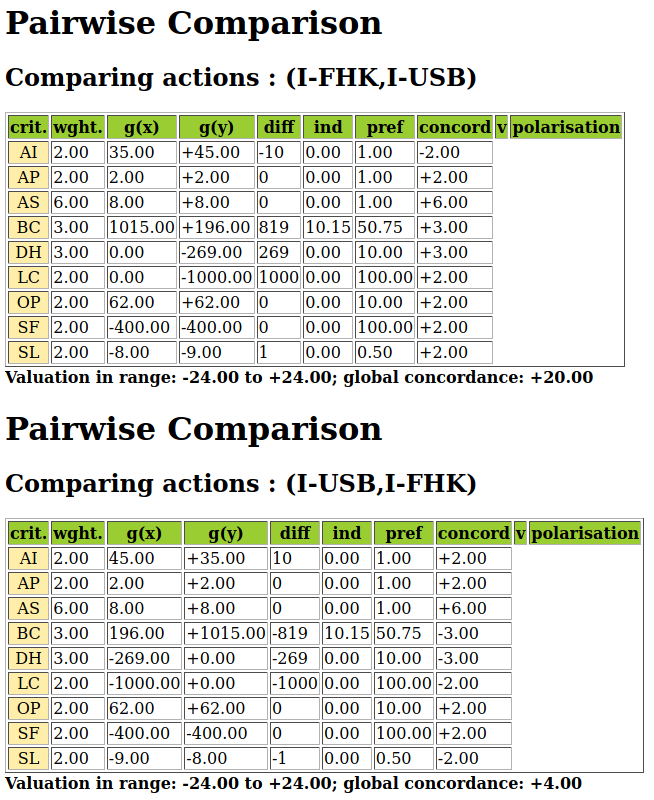
\includegraphics[width=7cm]{Figures/12-6-pairwiseComparison.png}
\caption{Comparing the first and second best-ranked study programs. The Köln alternative is performing \emph{at least as well as} the Saarbrücken alternative on all the performance criteria, except the \emph{Annual income} (of significance $2/24$). Conversely, the Saarbrücken alternative is clearly \emph{outperformed} from the geographical ($0/6$) as well as from the financial perspective ($2/6$)}
\label{fig:12.6}       % Give a unique label
\end{figure}
%\clearpage

In a similar way, one may finally compute a \emph{weak ranking} of all the potential study programs with the help of the \texttt{RankingByChoosingDigraph} constructor\index{RankingByChoosingDigraph@\texttt{RankingByChoosingDigraph} class}, that computes a bipolar ranking by conjointly \emph{best-choosing} and \emph{last-rejecting} \citep{BIS-1999}.
\begin{lstlisting}[caption={Weakly ranking by bipolar best-choosing and last-rejecting},label=list:12.6]
>>> from transitiveDigraphs import\
...               RankingByChoosingDigraph
>>> rbc = RankingByChoosingDigraph(dg)
>>> rbc.showRankingByChoosing()
    Ranking by Choosing and Rejecting
     1st ranked ['I-FHK'] 
       2nd ranked ['I-USB']
	 3rd ranked ['I-UHB']
	   4th ranked ['T-FHK']
	     5th ranked ['T-UD']
	     5th last ranked ['T-UD']
	   4th last ranked ['T-UHB', 'T-USB']
	 3rd last ranked ['T-FHM']
       2nd last ranked ['C-HKK']
     1st last ranked ['S-HKK']
\end{lstlisting}

In Listing~\vref{list:12.6}, we find confirmed that the \emph{Interpreter} studies appear all preferrred to the \emph{Translator} studies. Furthermore, the \emph{Interpreter} studies in Saarbrücken appear preferred to the same studies in Heidelberg. The Köln alternative is apparently the preferred one of all the \emph{Translater} studies. And, the \emph{Foreign Correspondent} and the \emph{Specialised Secretary} studies appear second-last and last ranked.

Yet, how \emph{robust} are our findings with respect to potential settings of the decision objectives' importance and the performance criteria significance?
		
\section{Robustness analysis}
\label{sec:12.4}

Alice considers her four decision objectives as being \emph{more or less} equally important. Here we have, however, allocated \emph{strictly equal} importance weights with \emph{strictly equi-significant} criteria per objective. How robust is our previous best choice recommendation when, now, we would consider the importance of the objectives and, hence, the significance of the respective performance criteria to be \emph{more or less uncertain}?

To answer this question, we will consider the respective criteria significance weights $w_j$ for $j=1,...,9$ to be \emph{triangular random variables} in the range 0 to $2w_j$ with mode = $w_j$. We may compute a corresponding $90\%$-\emph{confident} outranking digraph with the help of the \texttt{ConfidentBipolarOutrankingDigraph} constructor\index{ConfidentBipolarOutrankingDigraph@\texttt{ConfidentBipolarOutrankingDigraph} class} (see Chapter~\vref{sec:18}).
\begin{lstlisting}[caption={Computing the 90\% confident outranking digraph},label=list:12.7]
>>> from outrankingDigraphs import\
...         ConfidentBipolarOutrankingDigraph
>>> cdg = ConfidentBipolarOutrankingDigraph(t,\
...         distribution='triangular',confidence=90.0)
>>> cdg
  *------- Object instance description ------*
    Instance class       : ConfidentBipolarOutrankingDigraph
    Instance name        : rel_AliceChoice_CLT
    Actions              : 10
    Criteria             : 9
    Size                 : 44
    Valuation domain     : [-1.00;1.00]
    Uncertainty model    : triangular(a=0,b=2w) 
    Likelihood domain    : [-1.0;+1.0] 
    Confidence level     : 90.0% 
    Confident majority   : 14/24 (58.3%) 
    Determinateness (%)  : 68.19
\end{lstlisting}

Of the original 67 valid outranking situations, we retain 44 outranking situations as being $90\%$-confident (see Listing~\vref{list:12.7} Line 11). The corresponding $90\%$-confident \emph{qualified majority} of criteria significance amounts to $14/24 = 58.3\%$ (Line 16).  

Concerning now a $90\%$-confident best choice recommendation, we are lucky. 
\begin{lstlisting}[caption={Computing the $90\%$-confident best choice recommendation.},label=list:12.8]
>>> cdg.computeCondorcetWinners()
  ['I-FHK']
>>> cdg.showBestChoiceRecommendation()
  ***********************
  Best choice recommendation(s) (BCR)
   (in decreasing order of determinateness)   
   Credibility domain: [-1.00,1.00]
  === >> potential best choice(s)
   choice              : ['I-FHK','I-UHB','I-USB',
                          'T-FHK','T-FHM']
      independence        : 0.00
      dominance           : 0.42
      absorbency          : 0.00
      covering (%)        : 20.00
      determinateness (%) : 61.25
   - most credible action(s) = { 'I-FHK': 0.75, }
\end{lstlisting}

The \emph{Graduate Interpreter} studies in Köln remain indeed a 90\%-confident \Condorcet winner (see Fig.~\vref{fig:12.7} Line 2). Hence, the same study program also remains our 90\%-confident most credible best choice supported by a continual $18/24 (87.5\%)$ majority of the global criteria significance (see Lines 9-10 and 16 in Listing~\vref{list:12.8}).

When previously comparing the two best-ranked study programs (see Fig.~\vref{fig:12.6}), we have observed that \texttt{I-FHK} actually positively outranks \texttt{I-USB} on all four decision objectives. When admitting equi-significant criteria significances per objective, this outranking situation is hence valid independently of the importance weights Alice may allocate to each of her decision objectives. 

The \texttt{UnOpposedBipolarOutrankingDigraph} class constructor computes these \emph{unopposed} outranking situations (see Section~\vref{sec:19.5}).
\begin{lstlisting}[caption={Computing the unopposed outranking situations},label=list:12.9]
>>> from outrankingDigraphs import\
...                     UnOpposedBipolarOutrankingDigraph
>>> uop = UnOpposedBipolarOutrankingDigraph(t)
>>> uop
  *------- Object instance description ------*
   Instance class       : UnOpposedBipolarOutrankingDigraph
   Instance name        : AliceChoice_unopposed_outrankings
   Actions              : 10
   Criteria             : 9
   Size                 : 28
   Oppositeness (%)     : 58.21
   Determinateness (%)  : 62.94
   Valuation domain     : [-1.00;1.00]
>>> uop.isTransitive()
  True
\end{lstlisting}

We keep 28 out the 67 standard outranking situations, which leads to an \emph{oppositeness degree} of $(1.0 - 28/67) = 58.21\%$ (see Lines 10-11 in Listing~\vref{list:12.9}). Remarkable furthermore is that this unopposed outranking digraph \texttt{uop} is actually \emph{transitive}, i.e. modelling a \emph{partial ranking} of the study programs (Lines 14-15).

We may hence make use of the \texttt{exportGraphViz()} method of the \texttt{Transi\-tiveDigraph} class\index{TransitiveDigraph@\texttt{TransitiveDigraph} class} for drawing the corresponding partial ranking.
\begin{lstlisting}
>>> from transitiveDigraphs import TransitiveDigraph
>>> TransitiveDigraph.exportGraphViz(uop,\
...           fileName='choiceUnopposed')
  *---- exporting a dot file for GraphViz tools ---------*
   Exporting to choiceUnopposed.dot
   dot -Grankdir=TB -Tpng choiceUnopposed.dot -o choiceUnopposed.png
\end{lstlisting}
\begin{figure}[ht]
\sidecaption[t]
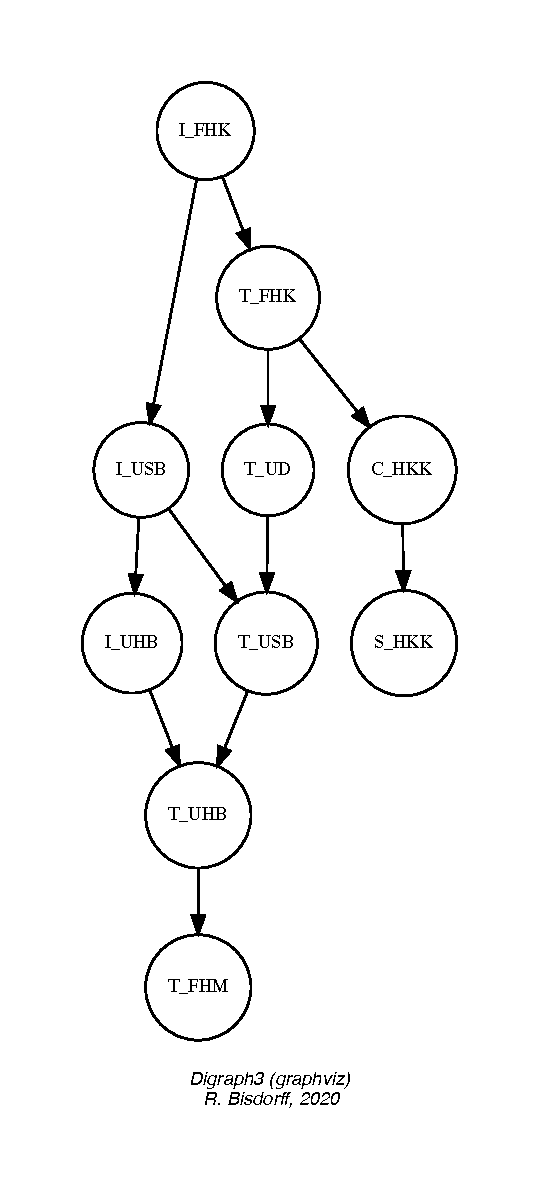
\includegraphics[width=6cm]{Figures/12-7-choiceUnopposed.pdf}
\caption{Unopposed partial ranking of the potential study programs. Again, when \emph{equi-signficant} performance criteria are assumed per decision objective, we observe in the Figure here that $I-FHK$ remains the stable best choice, \emph{independently} of the actual importance weights that Alice may wish to allocate to her four decision objectives}
\label{fig:12.7}       % Give a unique label
\end{figure}
%\clearpage

In view of her performance tableau shown in Fig.~\vref{fig:12.3}, \emph{Graduate Interpreter} studies at the Technical High School Köln, thus, represent definitely \textbf{Alice's very best choice}.

For further reading about the \Rubis \emph{Best Choice} methodology, one may consult in \citet{BIS-2015bestPoster} the study of a \emph{real decision aid case} about choosing a best poster in a scientific conference.
 
%%%%%%% The chapter bibliography
%\normallatexbib
\clearpage
%\phantomsection
%\addcontentsline{toc}{section}{Chapter Bibliography}
\bibliographystyle{spbasic}
%\typeout{}
\bibliography{03-backMatters/reference}
%\chapter{Alice's best choice: A selection case study}
\label{sec:12}
\abstract*{ The chapter presents a case study concerning the building of a best choice recommendation for Alice, a German student who wants some advice concerning the choice of her future University studies. We present Alice's performance tableau --potential foreign language study programs, her decision objectives, performance criteria and performance grades-- and build a best choice recommendation for her. A thorough robustness analysis confirms a very best choice.}

\abstract{ The chapter presents a case study concerning the building of a best choice recommendation for Alice, a German student who wants some advice concerning the choice of her future University studies. We present Alice's performance tableau --potential foreign language study programs, her decision objectives, performance criteria and performance grades-- and build a best choice recommendation for her. A thorough robustness analysis confirms a very best choice.}


\begin{figure}[ht]
\sidecaption

\includegraphics[width=4cm]{Figures/12-1-AliceF.png}
\caption{Alice D., 19 years old German student finishing her secondary studies in Köln (Germany), desires to undertake foreign languages studies.}
\label{fig:12.1}       % Give a unique label
\end{figure}

\noindent This case study is inspired by a multiple criteria decision analysis case study published by \citealp[pp. 1-17]{EIS-2001}.

\section{The decision problem}
\label{sec:12.1}

Alice will probably receive her "Abitur" with satisfactory and/or good marks and  wants to start her further studies thereafter. She would not mind staying in Köln, yet is ready to move elsewhere if necessary. The length of the higher studies do concern her, as she wants to earn her life as soon as possible.  Her parents however agree to financially support her study fees as well as her living costs during her studies.

Alice has already identified 10 potential study programs.
\begin{table}[h]
\caption{The potential study programs}
\label{tab:12.1}       % Give a unique label
\begin{center}
  %\begin{small}
    \begin{tabular}{l|l|l|l}
      \svhline\noalign{\smallskip}
      ID & Diploma & Institution & City\\
      \noalign{\smallskip}\hline\noalign{\smallskip}
      \texttt{T-UD}   & Qualified translator (T)  &   University (UD)               &  Düsseldorf\\
      \texttt{T-FHK}  & Qualified translator (T)  &   Higher Technical School (FHK) &  Köln\\
      \texttt{T-FHM}  & Qualified translator (T)  &   Higher Technical School (FHM) &  München\\
      \texttt{I-FHK}  & Graduate interpreter (I)  &   Higher Technical School (FHK) &  Köln\\
      \texttt{T-USB}  & Qualified translator (T)  &   University (USB)              &  Saarbrücken\\
      \texttt{I-USB}  & Graduate interpreter (I)  &   University (USB)              &  Saarbrücken\\
      \texttt{T-UHB}  & Qualified translator (T)  &   University (UHB)              &  Heidelberg\\
      \texttt{I-UHB}  & Graduate interpreter (I)  &   University (UHB)              &  Heidelberg\\
      \texttt{S-HKK}  & Specialized secretary (S) &   Chamber of Commerce (HKK)     &  Köln\\
      \texttt{C-HKK}  & Foreign correspondent (C) &   Chamber of Commerce (HKK)     &  Köln\\
      \noalign{\smallskip}\hline
    \end{tabular}
  %\end{small}
\end{center}
\end{table}

In Table~\vref{tab:12.1} we notice that Alice considers three \emph{Graduate Interpreter} studies (8 or 9 Semesters), respectively in Köln, in Saarbrücken or in Heidelberg; and five \emph{Qualified translator} studies (8 or 9 Semesters), respectively in Köln, in Düsseldorf, in Saarbrücken, in Heidelberg or in Munich. She also considers two short (4 Semesters) study programs at the Chamber of Commerce in Köln. 

Four \textbf{decision objectives} of more or less equal importance are guiding Alice's choice:
\begin{enumerate}[leftmargin=1cm,topsep=1pt]
\item \emph{maximize} the attractiveness of the study place (\texttt{GEO}),
\item \emph{maximize} the attractiveness of her further studies (\texttt{LEA}),
\item \emph{minimize}  her financial dependency on her parents (\texttt{FIN}),
\item \emph{maximize} her professional perspectives (\texttt{PRA}).
\end{enumerate}

The decision consequences Alice wishes to take into account for evaluating the potential study programs with respect to each of the four objectives are modelled by the following \emph{coherent family of criteria} \citep*{ROY-1991,ROY-1993}. Such a family of performance criteria verifies:
\begin{enumerate}[topsep=1pt]
\item \emph{Exhaustiveness}: No argument acceptable to Alice can be put forward to justify a preference in favour of study program $x$ versus program $y$  when $x$ and $y$ have the same performance level on each of the performance criteria;
\item \emph{Cohesiveness}: Alice recognizes that program $x$ must be preferred to program $y$ whenever the performance level of $x$ is significantly better than that of $y$ on one of the criteria of positive weight, performance levels of $x$ and $y$ being the same on each of the other criteria; 
\item \emph{Nonredundancy}: One of the above requirements is violated if one of the performance criteria is left out from the family.
\end{enumerate}

\begin{table}[h]
\caption{Alice's family of performance criteria}
\label{tab:12.2}       % Give a unique label
\begin{center}
  %\begin{small}
    \begin{tabular}{l|l|l|l|c}
      \svhline\noalign{\smallskip}
      ID & Name & Comment & Objective & Weight\\
      \noalign{\smallskip}\hline\noalign{\smallskip}
       \texttt{DH}  & Proximity  &  Distance in km to her home (min)      &   \texttt{GEO}    &     3\\
       \texttt{BC}  & Big City   &  Number of inhabitants (max)           &   \texttt{GEO}    &     3\\
       \   & \          &  \                                     &   \      &     \ \\
       \texttt{AS}  & Studies    &  Attractiveness of the studies (max)   &   \texttt{LEA}    &     6\\
       \   & \          &  \                                     &  \       &    \ \\
       \texttt{SF}  & Fees       &  Annual study fees (min)               &   \texttt{FIN}    &     2\\
       \texttt{LC}  & Living     &  Monthly living costs (min)            &   \texttt{FIN}    &     2\\
       \texttt{SL}  & Length     &  Length of the studies (min)           &   \texttt{FIN}    &     2\\
       \   &  \         &   \                                    &   \      &     \ \\
       \texttt{AP}  & Profession &  Attractiveness of the profession (max)&   \texttt{PRA}    &     2\\
       \texttt{AI}  & Income     &  Annual income after studying (max)    &   \texttt{PRA}    &     2\\
       \texttt{PR}  & Prestige   &  Occupational prestige (max)           &   \texttt{PRA}    &     2\\
      \noalign{\smallskip}\hline
    \end{tabular}
  %\end{small}
\end{center}
\end{table}

Within each decision objective, the performance criteria are considered to be \emph{equisignificant}. Hence, the four decision objectives get a same \emph{importance weight} of $6$ (see Table~\vref{tab:12.2} Column 5).

\section{The performance tableau}
\label{sec:12.2}

The actual evaluations of Alice's potential study programs are stored in a file named \texttt{AliceChoice.py} of \texttt{PerformanceTableau} format \footnote{The performance tableau \texttt{AliceChoice.py} may be found in the \texttt{examples} directory of the \Digraph resources\citep{BIS-2021}.}.
\begin{lstlisting}[caption={Alice's performance tableau},label=list:12.1]
>>> from perfTabs import PerformanceTableau
>>> t = PerformanceTableau('AliceChoice')
>>> t.showObjectives()
  *------ decision objectives -------"
    GEO: Geographical aspect
     DH Distance to parent's home 3
     BC Number of inhabitants     3
     Total weight: 6 (2 criteria)
    LEA: Learning aspect
     AS Attractiveness of the study program 6
     Total weight: 6.00 (1 criteria)
    FIN: Financial aspect
     SF Annual registration fees 2
     LC Monthly living costs     2
     SL Study time               2
     Total weight: 6.00 (3 criteria)
    PRA: Professional aspect
     AP Attractiveness of the profession          2
     AI Annual professional income after studying 2
     OP Occupational Prestige                     2
     Total weight: 6.00 (3 criteria)
\end{lstlisting}

Details of the performance criteria may be consulted in the browser view below.\index{showHTMCriteria@\texttt{showHTMCriteria()}}
\begin{lstlisting}
>>> t.showHTMLCriteria()
\end{lstlisting}
\begin{figure}[ht]
%\sidecaption
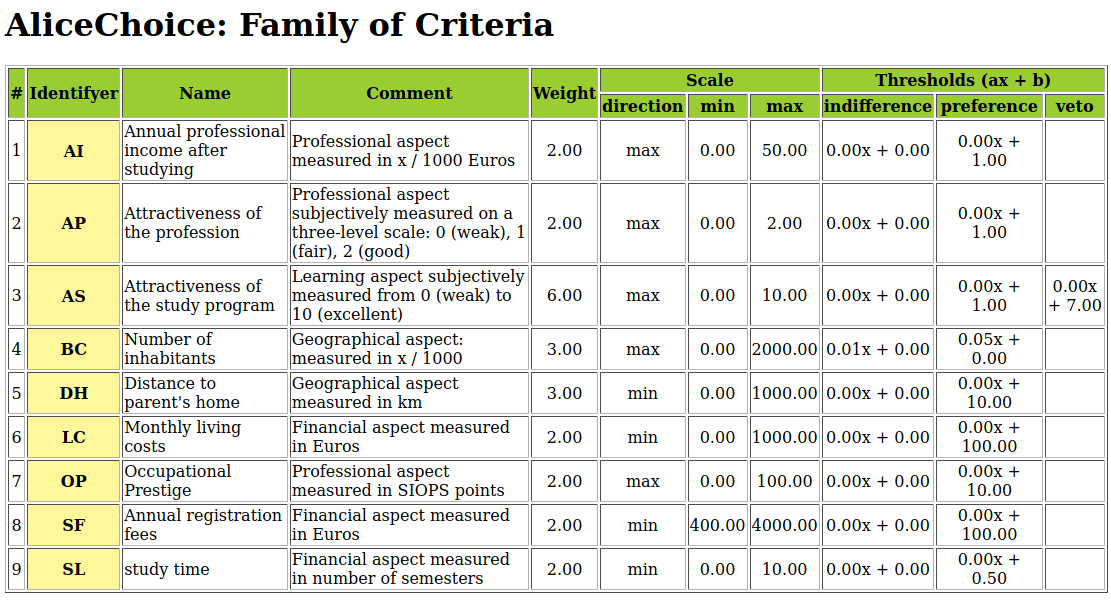
\includegraphics[width=\hsize]{Figures/12-2-aliceCriteria.png}
\caption{Alice's performance criteria}
\label{fig:12.2}       % Give a unique label
\end{figure}

It is worthwhile noticing in Fig.~\vref{fig:12.2} that, on her subjective attractiveness scale of the study programs (criterion \texttt{AS}), Alice considers a performance differences of 7 points to be \emph{considerable} and triggering, the case given, an outranking polarisation \citep{BIS-2013}. Notice also the proportional \emph{indifference} ($1\%$) and \emph{preference} ($5\%$) discrimination thresholds shown on criterion \texttt{BC} (number of inhabitants).

Alice is subjectively evaluating the \emph{Attractiveness} of the studies (criterion \texttt{AS}) on an ordinal scale from \emph{weak} ($0$) to \emph{excellent} ($10$). Similarly, she is subjectively evaluating the \emph{Attractiveness} of the respective professions (criterion \texttt{AP}) on a three level ordinal scale from \emph{weak} ($0$), \emph{fair} ($1$) to \emph{good} ($2$). Considering the \emph{Occupational Prestige} (criterion \texttt{OP}), she looked up the SIOPS \footnote{Standard International Occupational Prestige Scale \citep*{GAN-1996}.}. All the other evaluation data she found on the internet.

In the \emph{heatmap view} shown in Fig.~\vref{fig:12.3}, we may now consult Alice's performance gradings.
\begin{lstlisting}
>>> t.showHTMLPerformanceHeatmap(\
...       colorLevels=5,Correlations=True,ndigits=0)
\end{lstlisting}
\begin{figure}[ht]
%\sidecaption
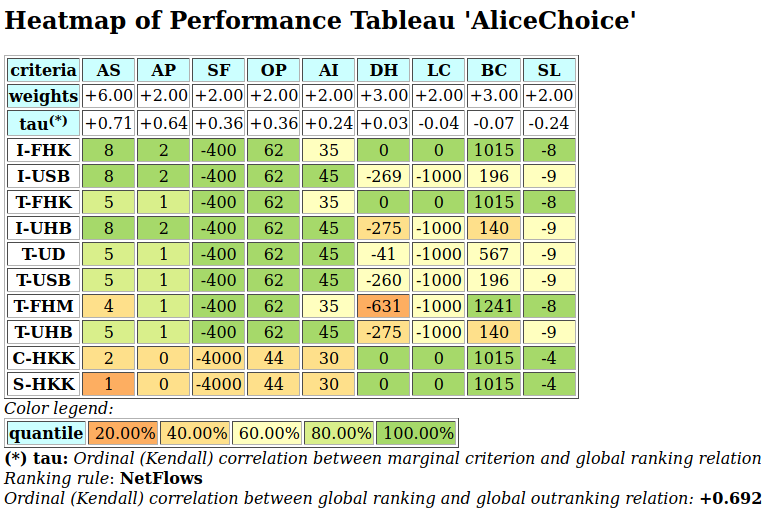
\includegraphics[width=\hsize]{Figures/12-3-aliceHeatmap.png}
\caption{Heatmap of Alice's performance tableau}
\label{fig:12.3}       % Give a unique label
\end{figure}

Her ten potential study programs are ordered with the \NetFlows ranking rule applied to the corresponding bipolar-valued outranking digraph (see Section~\vref{sec:8.3}). \emph{Graduate interpreter} studies in Köln (\texttt{I-FHK}) or Saarbrücken (\texttt{I-USB}), followed by \emph{Qualified Translator} studies in Köln (\texttt{T-FHK}) appear to be Alice's most preferred alternatives. The least attractive for her appear to be studies at the Chamber of Commerce of Köln (\texttt{C-HKK}, \texttt{S-HKK}). Notice by the way that evaluations on performance criteria to be \emph{minimized}, like \emph{Distance to Home} (criterion \texttt{DH}) or \emph{Study time} (criterion \texttt{SL}), are registered as \emph{negative} values, so that smaller measures are, in this case, preferred to larger ones.

It is finally interesting to observe in Fig.~\vref{fig:12.3} (third row) that the \emph{most significant} performance criteria, appear to be for Alice, on the one side, the \emph{Attractiveness} of the study program (criterion \texttt{AS}, tau = $+0.72$) followed by the \emph{Attractiveness} of the future profession (criterion \texttt{AP}, tau = $+0.62$). On the other side, \emph{Study times} (criterion \texttt{SL}, tau = $-0.24$), \emph{Big city} (criterion \texttt{BC}, tau = $-0.07$) as well as \emph{Monthly living costs} (criterion \texttt{LC}, tau = $-0.04$) appear to be \emph{not so significant} (see Chapter~\vref{sec:16}).

\section{Building a best choice recommendation}
\label{sec:12.3}

Let us now have a look at the resulting pairwise outranking situations.
\begin{lstlisting}[caption={Computing Alice's outranking digraph},label=list:12.2]
>>> from outrankingDigraphs import BipolarOutrankingDigraph
>>> dg = BipolarOutrankingDigraph(t) 
>>> dg
  *------- Object instance description ------*
   Instance class      : BipolarOutrankingDigraph
   Instance name       : rel_AliceChoice
   Actions             : 10
   Criteria            : 9
   Size                : 67
   Determinateness (%) : 73.91
   Valuation domain    : [-1.00;1.00]
>>> dg.computeSymmetryDegree(Comments=True)
  Symmetry degree of graph <rel_AliceChoice> : 0.49
\end{lstlisting}

From Alice's performance tableau we obtain in the digraph \texttt{dg}  67 positively validated pairwise outranking situations, supported by a $74\%$ majority of criteria significance (see Lines 9-10 in Listing~\vref{list:12.2}).

Due to the poorly discriminating performance evaluations, nearly half of these outranking situations (see Line 12) are \emph{symmetric} and reveal actually \emph{more or less indifference} situations between the potential study programs. This is well illustrated in the \emph{relation map} of the outranking digraph shown in Fig.~\vref{fig:12.4}.
\begin{figure}[ht]
%\sidecaption
\includegraphics[width=10cm]{Figures/12-4-aliceRelationmap.png}
\caption{\Copeland ranked outranking relation map}
\label{fig:12.4}       % Give a unique label
\end{figure}
\begin{lstlisting}
>>> dg.showHTMLRelationMap(\
...           tableTitle='Outranking relation map',\
...           rankingRule='Copeland')
\end{lstlisting}

We have mentioned that Alice considers a performance difference of $7$ points on the \emph{Attractiveness of studies} criterion \texttt{AS} to be considerable which triggers, the case given, a potential polarisation of the outranking characteristics. In Fig.~\vref{fig:12.4}, these polarisations appear in the last column and last row. We may inspect the occurrence of such polarisations with the \texttt{showPolarisations()} method. \index{showPolarisations@\texttt{showPolarisations()}}
\begin{lstlisting}[caption={Polarised outranking situations},label=list:12.3]
>>> dg.showPolarisations()
  *----  Negative polarisations ----*
   number of negative polarisations : 3 
    1: r(S-HKK >= I-FHK) = -0.17
     criterion: AS
     Considerable performance difference : -7.00
     Veto discrimination threshold       : -7.00
     Polarisation: r(S-HKK >= I-FHK) = -0.17 ==> -1.00
    2: r(S-HKK >= I-USB) = -0.17
     criterion: AS
     Considerable performance difference : -7.00
     Veto discrimination threshold       : -7.00
     Polarisation: r(S-HKK >= I-USB) = -0.17 ==> -1.00
    3: r(S-HKK >= I-UHB) = -0.17
     criterion: AS
     Considerable performance difference : -7.00
     Veto discrimination threshold       : -7.00
     Polarisation: r(S-HKK >= I-UHB) = -0.17 ==> -1.00
  *----  Positive polarisations ----*
   number of positive polarisations: 3 
    1: r(I-FHK >= S-HKK) = 0.83
     criterion: AS
     Considerable performance difference : 7.00
     Counter-veto threshold              : 7.00
     Polarisation: r(I-FHK >= S-HKK) = 0.83 ==> +1.00
    2: r(I-USB >= S-HKK) = 0.17
     criterion: AS
     Considerable performance difference : 7.00
     Counter-veto threshold              : 7.00
     Polarisation: r(I-USB >= S-HKK) = 0.17 ==> +1.00
    3: r(I-UHB >= S-HKK) = 0.17
     criterion: AS
     Considerable performance difference : 7.00
     Counter-veto threshold              : 7.00
     Polarisation: r(I-UHB >= S-HKK) = 0.17 ==> +1.00
\end{lstlisting}

In Listing~\vref{list:12.3}, we see that \emph{considerable} performance differences concerning the \emph{Attractiveness of the studies} (\texttt{AS} criterion) are indeed observed between the \emph{Specialised Secretary} study programm offered in Köln and the \emph{Graduate Interpreter} study programs offered in Köln, Saarbrücken and Heidelberg. They polarise, hence, three \emph{more or less invalid} outranking situations to \emph{certainly invalid} (Lines 8, 13, 18) and corresponding three \emph{more or less valid} converse outranking situations to \emph{certainly valid} ones (Lines 25, 30, 35). 

We may finally notice in the relation map, shown in Fig.~\vref{fig:12.4}, that the four best-ranked study programs, \texttt{I-FHK}, \texttt{I-USB}, \texttt{I-UHB} and \texttt{T-FHK},  are in fact \Condorcet winners (see Listing~\vref{list:12.4} Line 2), i.e. they are all four \emph{indifferent} one of the other \textbf{and} positively \emph{outranking} all other alternatives, a result confirmed in Listing~\vref{list:12.4} below by our \Rubis best choice recommendation \citep*{BIS-2008a}.
\begin{lstlisting}[caption={Alice's best choice recommendation},label=list:12.4]
>>> dg.computeCondorcetWinners()
  ['I-FHK', 'I-UHB', 'I-USB', 'T-FHK'] 
>>> dg.showBestChoiceRecommendation()
  Best choice recommendation(s) (BCR)
    (in decreasing order of determinateness)   
    Credibility domain: [-1.00,1.00]
   === >> potential best choice(s)
   choice                : ['I-FHK','I-UHB','I-USB','T-FHK']
     independence        : 0.17
     dominance           : 0.08
     absorbency          : -0.83
     covering (%)        : 62.50
     determinateness (%) : 68.75
     most credible action(s) = {'I-FHK': 0.75,'T-FHK': 0.17,
                                'I-USB': 0.17,'I-UHB': 0.17}
   === >> potential worst choice(s) 
   choice                : ['C-HKK', 'S-HKK']
     independence        : 0.50
     dominance           : -0.83
     absorbency          : 0.17
     covered (%)         : 100.00
     determinateness (%) : 58.33
     most credible action(s) = {'S-HKK': 0.17,'C-HKK': 0.17}
\end{lstlisting}

Most credible best choice among the four best-ranked study programs eventually becomes the \emph{Graduate Interpreter} study program at the Technical High School in Köln (see Line 14) supported by a $(0.75 + 1)/2.0 \,=\,87.5\% (18/24)$ majority of global criteria significance \footnote{See Section~\vref{sec:17.6} on solving \Berge kernel equation systems.}.

In the relation map, shown in Fig.~\vref{fig:12.4}, we see in the left lower corner that the \emph{asymmetric part} of the outranking relation, i.e. the corresponding \emph{strict} outranking relation, is actually \emph{transitive} (see Line 2 below). Hence, a \emph{graphviz} drawing of its \emph{skeleton}, oriented by the previous \emph{best}, respectively \emph{worst} choice, may well illustrate our \emph{best choice recommendation}.
\begin{lstlisting}[caption={Alice's strict best choice recommendation},label=list:12.5]
>>> dgcd = ~(-dg)
>>> dgcd.isTransitive()
    True
>>> dgcd.closeTransitive(Reverse=True,InSite=True)
>>> dgcd.exportGraphViz('aliceBestChoice',\
...                     bestChoice=['I-FHK'],\
...                     worstChoice=['S-HKK','C-HKK'])
  *---- exporting a dot file for GraphViz tools ---------*
   Exporting to aliceBestChoice.dot
   dot -Grankdir=BT -Tpng aliceBestChoice.dot -o aliceBestChoice.png
\end{lstlisting}
\begin{figure}[ht]
\sidecaption[t]
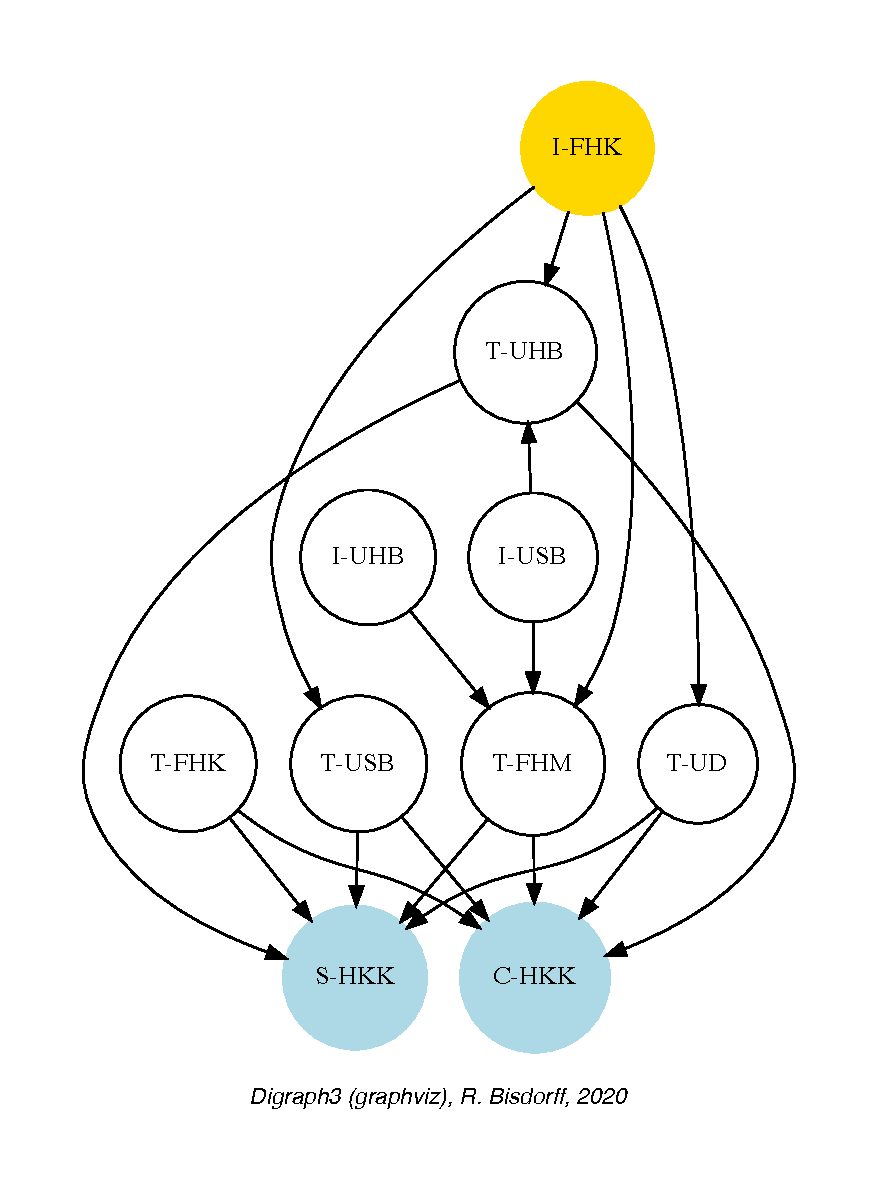
\includegraphics[width=7cm]{Figures/12-5-aliceBestChoice.pdf}
\caption{In Alice's best choice recommendation, we notice that the \emph{Graduate Interpreter} studies come first, followed by the \emph{Qualified Translator} studies. Last come the \emph{Chamber of Commerce}'s specialised studies. This confirms again the high significance that Alice attaches to the \emph{attractiveness} of her further studies and of her future profession (see criteria \texttt{AS} and \texttt{AP} in Fig.~\vref{fig:12.3})}
\label{fig:12.5}       % Give a unique label
\end{figure}

Let us now, for instance, check the pairwise outranking situations observed between the first and second-ranked alternative, i.e. \emph{Garduate Interpreter} studies in Köln versus \emph{Graduate Interpreter} studies in Saabrücken (see \texttt{I-FHK} and \texttt{I-USB} in Fig.~\vref{fig:12.3}).
\begin{lstlisting}
>>> dg.showHTMLPairwiseOutrankings('I-FHK','I-USB')
\end{lstlisting}
\begin{figure}[ht]
\sidecaption[t]
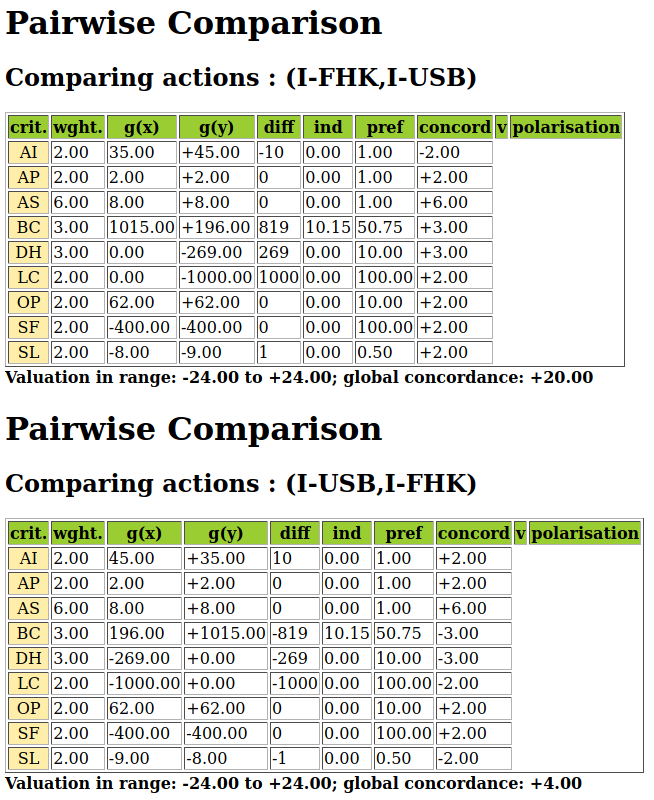
\includegraphics[width=7cm]{Figures/12-6-pairwiseComparison.png}
\caption{Comparing the first and second best-ranked study programs. The Köln alternative is performing \emph{at least as well as} the Saarbrücken alternative on all the performance criteria, except the \emph{Annual income} (of significance $2/24$). Conversely, the Saarbrücken alternative is clearly \emph{outperformed} from the geographical ($0/6$) as well as from the financial perspective ($2/6$)}
\label{fig:12.6}       % Give a unique label
\end{figure}
%\clearpage

In a similar way, one may finally compute a \emph{weak ranking} of all the potential study programs with the help of the \texttt{RankingByChoosingDigraph} constructor\index{RankingByChoosingDigraph@\texttt{RankingByChoosingDigraph} class}, that computes a bipolar ranking by conjointly \emph{best-choosing} and \emph{last-rejecting} \citep{BIS-1999}.
\begin{lstlisting}[caption={Weakly ranking by bipolar best-choosing and last-rejecting},label=list:12.6]
>>> from transitiveDigraphs import\
...               RankingByChoosingDigraph
>>> rbc = RankingByChoosingDigraph(dg)
>>> rbc.showRankingByChoosing()
    Ranking by Choosing and Rejecting
     1st ranked ['I-FHK'] 
       2nd ranked ['I-USB']
	 3rd ranked ['I-UHB']
	   4th ranked ['T-FHK']
	     5th ranked ['T-UD']
	     5th last ranked ['T-UD']
	   4th last ranked ['T-UHB', 'T-USB']
	 3rd last ranked ['T-FHM']
       2nd last ranked ['C-HKK']
     1st last ranked ['S-HKK']
\end{lstlisting}

In Listing~\vref{list:12.6}, we find confirmed that the \emph{Interpreter} studies appear all preferrred to the \emph{Translator} studies. Furthermore, the \emph{Interpreter} studies in Saarbrücken appear preferred to the same studies in Heidelberg. The Köln alternative is apparently the preferred one of all the \emph{Translater} studies. And, the \emph{Foreign Correspondent} and the \emph{Specialised Secretary} studies appear second-last and last ranked.

Yet, how \emph{robust} are our findings with respect to potential settings of the decision objectives' importance and the performance criteria significance?
		
\section{Robustness analysis}
\label{sec:12.4}

Alice considers her four decision objectives as being \emph{more or less} equally important. Here we have, however, allocated \emph{strictly equal} importance weights with \emph{strictly equi-significant} criteria per objective. How robust is our previous best choice recommendation when, now, we would consider the importance of the objectives and, hence, the significance of the respective performance criteria to be \emph{more or less uncertain}?

To answer this question, we will consider the respective criteria significance weights $w_j$ for $j=1,...,9$ to be \emph{triangular random variables} in the range 0 to $2w_j$ with mode = $w_j$. We may compute a corresponding $90\%$-\emph{confident} outranking digraph with the help of the \texttt{ConfidentBipolarOutrankingDigraph} constructor\index{ConfidentBipolarOutrankingDigraph@\texttt{ConfidentBipolarOutrankingDigraph} class} (see Chapter~\vref{sec:18}).
\begin{lstlisting}[caption={Computing the 90\% confident outranking digraph},label=list:12.7]
>>> from outrankingDigraphs import\
...         ConfidentBipolarOutrankingDigraph
>>> cdg = ConfidentBipolarOutrankingDigraph(t,\
...         distribution='triangular',confidence=90.0)
>>> cdg
  *------- Object instance description ------*
    Instance class       : ConfidentBipolarOutrankingDigraph
    Instance name        : rel_AliceChoice_CLT
    Actions              : 10
    Criteria             : 9
    Size                 : 44
    Valuation domain     : [-1.00;1.00]
    Uncertainty model    : triangular(a=0,b=2w) 
    Likelihood domain    : [-1.0;+1.0] 
    Confidence level     : 90.0% 
    Confident majority   : 14/24 (58.3%) 
    Determinateness (%)  : 68.19
\end{lstlisting}

Of the original 67 valid outranking situations, we retain 44 outranking situations as being $90\%$-confident (see Listing~\vref{list:12.7} Line 11). The corresponding $90\%$-confident \emph{qualified majority} of criteria significance amounts to $14/24 = 58.3\%$ (Line 16).  

Concerning now a $90\%$-confident best choice recommendation, we are lucky. 
\begin{lstlisting}[caption={Computing the $90\%$-confident best choice recommendation.},label=list:12.8]
>>> cdg.computeCondorcetWinners()
  ['I-FHK']
>>> cdg.showBestChoiceRecommendation()
  ***********************
  Best choice recommendation(s) (BCR)
   (in decreasing order of determinateness)   
   Credibility domain: [-1.00,1.00]
  === >> potential best choice(s)
   choice              : ['I-FHK','I-UHB','I-USB',
                          'T-FHK','T-FHM']
      independence        : 0.00
      dominance           : 0.42
      absorbency          : 0.00
      covering (%)        : 20.00
      determinateness (%) : 61.25
   - most credible action(s) = { 'I-FHK': 0.75, }
\end{lstlisting}

The \emph{Graduate Interpreter} studies in Köln remain indeed a 90\%-confident \Condorcet winner (see Fig.~\vref{fig:12.7} Line 2). Hence, the same study program also remains our 90\%-confident most credible best choice supported by a continual $18/24 (87.5\%)$ majority of the global criteria significance (see Lines 9-10 and 16 in Listing~\vref{list:12.8}).

When previously comparing the two best-ranked study programs (see Fig.~\vref{fig:12.6}), we have observed that \texttt{I-FHK} actually positively outranks \texttt{I-USB} on all four decision objectives. When admitting equi-significant criteria significances per objective, this outranking situation is hence valid independently of the importance weights Alice may allocate to each of her decision objectives. 

The \texttt{UnOpposedBipolarOutrankingDigraph} class constructor computes these \emph{unopposed} outranking situations (see Section~\vref{sec:19.5}).
\begin{lstlisting}[caption={Computing the unopposed outranking situations},label=list:12.9]
>>> from outrankingDigraphs import\
...                     UnOpposedBipolarOutrankingDigraph
>>> uop = UnOpposedBipolarOutrankingDigraph(t)
>>> uop
  *------- Object instance description ------*
   Instance class       : UnOpposedBipolarOutrankingDigraph
   Instance name        : AliceChoice_unopposed_outrankings
   Actions              : 10
   Criteria             : 9
   Size                 : 28
   Oppositeness (%)     : 58.21
   Determinateness (%)  : 62.94
   Valuation domain     : [-1.00;1.00]
>>> uop.isTransitive()
  True
\end{lstlisting}

We keep 28 out the 67 standard outranking situations, which leads to an \emph{oppositeness degree} of $(1.0 - 28/67) = 58.21\%$ (see Lines 10-11 in Listing~\vref{list:12.9}). Remarkable furthermore is that this unopposed outranking digraph \texttt{uop} is actually \emph{transitive}, i.e. modelling a \emph{partial ranking} of the study programs (Lines 14-15).

We may hence make use of the \texttt{exportGraphViz()} method of the \texttt{Transi\-tiveDigraph} class\index{TransitiveDigraph@\texttt{TransitiveDigraph} class} for drawing the corresponding partial ranking.
\begin{lstlisting}
>>> from transitiveDigraphs import TransitiveDigraph
>>> TransitiveDigraph.exportGraphViz(uop,\
...           fileName='choiceUnopposed')
  *---- exporting a dot file for GraphViz tools ---------*
   Exporting to choiceUnopposed.dot
   dot -Grankdir=TB -Tpng choiceUnopposed.dot -o choiceUnopposed.png
\end{lstlisting}
\begin{figure}[ht]
\sidecaption[t]
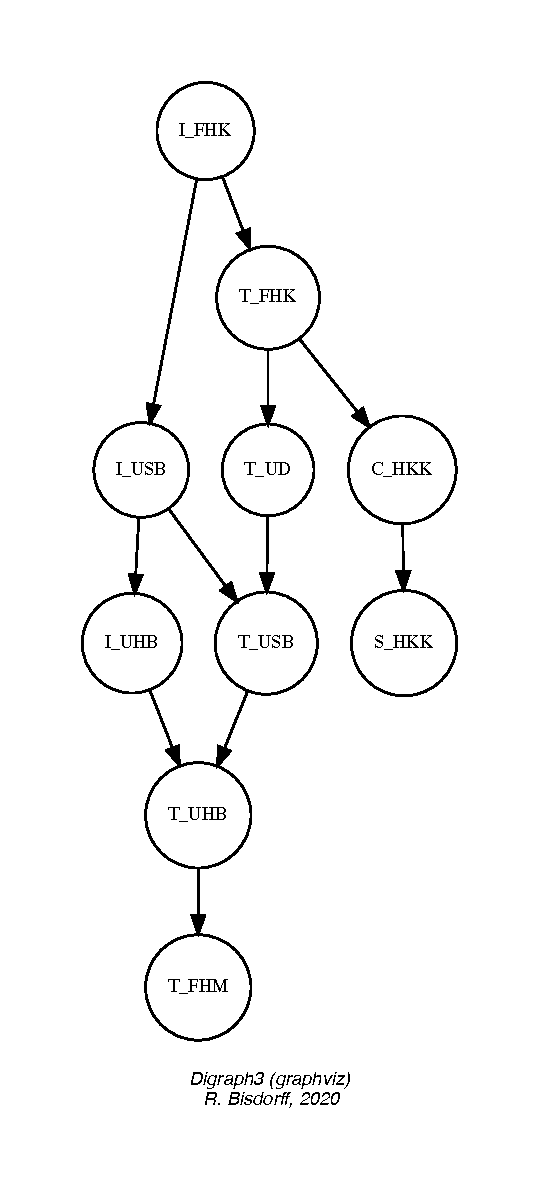
\includegraphics[width=6cm]{Figures/12-7-choiceUnopposed.pdf}
\caption{Unopposed partial ranking of the potential study programs. Again, when \emph{equi-signficant} performance criteria are assumed per decision objective, we observe in the Figure here that $I-FHK$ remains the stable best choice, \emph{independently} of the actual importance weights that Alice may wish to allocate to her four decision objectives}
\label{fig:12.7}       % Give a unique label
\end{figure}
%\clearpage

In view of her performance tableau shown in Fig.~\vref{fig:12.3}, \emph{Graduate Interpreter} studies at the Technical High School Köln, thus, represent definitely \textbf{Alice's very best choice}.

For further reading about the \Rubis \emph{Best Choice} methodology, one may consult in \citet{BIS-2015bestPoster} the study of a \emph{real decision aid case} about choosing a best poster in a scientific conference.
 
%%%%%%% The chapter bibliography
%\normallatexbib
\clearpage
%\phantomsection
%\addcontentsline{toc}{section}{Chapter Bibliography}
\bibliographystyle{spbasic}
%\typeout{}
\bibliography{03-backMatters/reference}
%\chapter{Alice's best choice: A selection case study}
\label{sec:12}
\abstract*{ The chapter presents a case study concerning the building of a best choice recommendation for Alice, a German student who wants some advice concerning the choice of her future University studies. We present Alice's performance tableau --potential foreign language study programs, her decision objectives, performance criteria and performance grades-- and build a best choice recommendation for her. A thorough robustness analysis confirms a very best choice.}

\abstract{ The chapter presents a case study concerning the building of a best choice recommendation for Alice, a German student who wants some advice concerning the choice of her future University studies. We present Alice's performance tableau --potential foreign language study programs, her decision objectives, performance criteria and performance grades-- and build a best choice recommendation for her. A thorough robustness analysis confirms a very best choice.}


\begin{figure}[ht]
\sidecaption

\includegraphics[width=4cm]{Figures/12-1-AliceF.png}
\caption{Alice D., 19 years old German student finishing her secondary studies in Köln (Germany), desires to undertake foreign languages studies.}
\label{fig:12.1}       % Give a unique label
\end{figure}

\noindent This case study is inspired by a multiple criteria decision analysis case study published by \citealp[pp. 1-17]{EIS-2001}.

\section{The decision problem}
\label{sec:12.1}

Alice will probably receive her "Abitur" with satisfactory and/or good marks and  wants to start her further studies thereafter. She would not mind staying in Köln, yet is ready to move elsewhere if necessary. The length of the higher studies do concern her, as she wants to earn her life as soon as possible.  Her parents however agree to financially support her study fees as well as her living costs during her studies.

Alice has already identified 10 potential study programs.
\begin{table}[h]
\caption{The potential study programs}
\label{tab:12.1}       % Give a unique label
\begin{center}
  %\begin{small}
    \begin{tabular}{l|l|l|l}
      \svhline\noalign{\smallskip}
      ID & Diploma & Institution & City\\
      \noalign{\smallskip}\hline\noalign{\smallskip}
      \texttt{T-UD}   & Qualified translator (T)  &   University (UD)               &  Düsseldorf\\
      \texttt{T-FHK}  & Qualified translator (T)  &   Higher Technical School (FHK) &  Köln\\
      \texttt{T-FHM}  & Qualified translator (T)  &   Higher Technical School (FHM) &  München\\
      \texttt{I-FHK}  & Graduate interpreter (I)  &   Higher Technical School (FHK) &  Köln\\
      \texttt{T-USB}  & Qualified translator (T)  &   University (USB)              &  Saarbrücken\\
      \texttt{I-USB}  & Graduate interpreter (I)  &   University (USB)              &  Saarbrücken\\
      \texttt{T-UHB}  & Qualified translator (T)  &   University (UHB)              &  Heidelberg\\
      \texttt{I-UHB}  & Graduate interpreter (I)  &   University (UHB)              &  Heidelberg\\
      \texttt{S-HKK}  & Specialized secretary (S) &   Chamber of Commerce (HKK)     &  Köln\\
      \texttt{C-HKK}  & Foreign correspondent (C) &   Chamber of Commerce (HKK)     &  Köln\\
      \noalign{\smallskip}\hline
    \end{tabular}
  %\end{small}
\end{center}
\end{table}

In Table~\vref{tab:12.1} we notice that Alice considers three \emph{Graduate Interpreter} studies (8 or 9 Semesters), respectively in Köln, in Saarbrücken or in Heidelberg; and five \emph{Qualified translator} studies (8 or 9 Semesters), respectively in Köln, in Düsseldorf, in Saarbrücken, in Heidelberg or in Munich. She also considers two short (4 Semesters) study programs at the Chamber of Commerce in Köln. 

Four \textbf{decision objectives} of more or less equal importance are guiding Alice's choice:
\begin{enumerate}[leftmargin=1cm,topsep=1pt]
\item \emph{maximize} the attractiveness of the study place (\texttt{GEO}),
\item \emph{maximize} the attractiveness of her further studies (\texttt{LEA}),
\item \emph{minimize}  her financial dependency on her parents (\texttt{FIN}),
\item \emph{maximize} her professional perspectives (\texttt{PRA}).
\end{enumerate}

The decision consequences Alice wishes to take into account for evaluating the potential study programs with respect to each of the four objectives are modelled by the following \emph{coherent family of criteria} \citep*{ROY-1991,ROY-1993}. Such a family of performance criteria verifies:
\begin{enumerate}[topsep=1pt]
\item \emph{Exhaustiveness}: No argument acceptable to Alice can be put forward to justify a preference in favour of study program $x$ versus program $y$  when $x$ and $y$ have the same performance level on each of the performance criteria;
\item \emph{Cohesiveness}: Alice recognizes that program $x$ must be preferred to program $y$ whenever the performance level of $x$ is significantly better than that of $y$ on one of the criteria of positive weight, performance levels of $x$ and $y$ being the same on each of the other criteria; 
\item \emph{Nonredundancy}: One of the above requirements is violated if one of the performance criteria is left out from the family.
\end{enumerate}

\begin{table}[h]
\caption{Alice's family of performance criteria}
\label{tab:12.2}       % Give a unique label
\begin{center}
  %\begin{small}
    \begin{tabular}{l|l|l|l|c}
      \svhline\noalign{\smallskip}
      ID & Name & Comment & Objective & Weight\\
      \noalign{\smallskip}\hline\noalign{\smallskip}
       \texttt{DH}  & Proximity  &  Distance in km to her home (min)      &   \texttt{GEO}    &     3\\
       \texttt{BC}  & Big City   &  Number of inhabitants (max)           &   \texttt{GEO}    &     3\\
       \   & \          &  \                                     &   \      &     \ \\
       \texttt{AS}  & Studies    &  Attractiveness of the studies (max)   &   \texttt{LEA}    &     6\\
       \   & \          &  \                                     &  \       &    \ \\
       \texttt{SF}  & Fees       &  Annual study fees (min)               &   \texttt{FIN}    &     2\\
       \texttt{LC}  & Living     &  Monthly living costs (min)            &   \texttt{FIN}    &     2\\
       \texttt{SL}  & Length     &  Length of the studies (min)           &   \texttt{FIN}    &     2\\
       \   &  \         &   \                                    &   \      &     \ \\
       \texttt{AP}  & Profession &  Attractiveness of the profession (max)&   \texttt{PRA}    &     2\\
       \texttt{AI}  & Income     &  Annual income after studying (max)    &   \texttt{PRA}    &     2\\
       \texttt{PR}  & Prestige   &  Occupational prestige (max)           &   \texttt{PRA}    &     2\\
      \noalign{\smallskip}\hline
    \end{tabular}
  %\end{small}
\end{center}
\end{table}

Within each decision objective, the performance criteria are considered to be \emph{equisignificant}. Hence, the four decision objectives get a same \emph{importance weight} of $6$ (see Table~\vref{tab:12.2} Column 5).

\section{The performance tableau}
\label{sec:12.2}

The actual evaluations of Alice's potential study programs are stored in a file named \texttt{AliceChoice.py} of \texttt{PerformanceTableau} format \footnote{The performance tableau \texttt{AliceChoice.py} may be found in the \texttt{examples} directory of the \Digraph resources\citep{BIS-2021}.}.
\begin{lstlisting}[caption={Alice's performance tableau},label=list:12.1]
>>> from perfTabs import PerformanceTableau
>>> t = PerformanceTableau('AliceChoice')
>>> t.showObjectives()
  *------ decision objectives -------"
    GEO: Geographical aspect
     DH Distance to parent's home 3
     BC Number of inhabitants     3
     Total weight: 6 (2 criteria)
    LEA: Learning aspect
     AS Attractiveness of the study program 6
     Total weight: 6.00 (1 criteria)
    FIN: Financial aspect
     SF Annual registration fees 2
     LC Monthly living costs     2
     SL Study time               2
     Total weight: 6.00 (3 criteria)
    PRA: Professional aspect
     AP Attractiveness of the profession          2
     AI Annual professional income after studying 2
     OP Occupational Prestige                     2
     Total weight: 6.00 (3 criteria)
\end{lstlisting}

Details of the performance criteria may be consulted in the browser view below.\index{showHTMCriteria@\texttt{showHTMCriteria()}}
\begin{lstlisting}
>>> t.showHTMLCriteria()
\end{lstlisting}
\begin{figure}[ht]
%\sidecaption
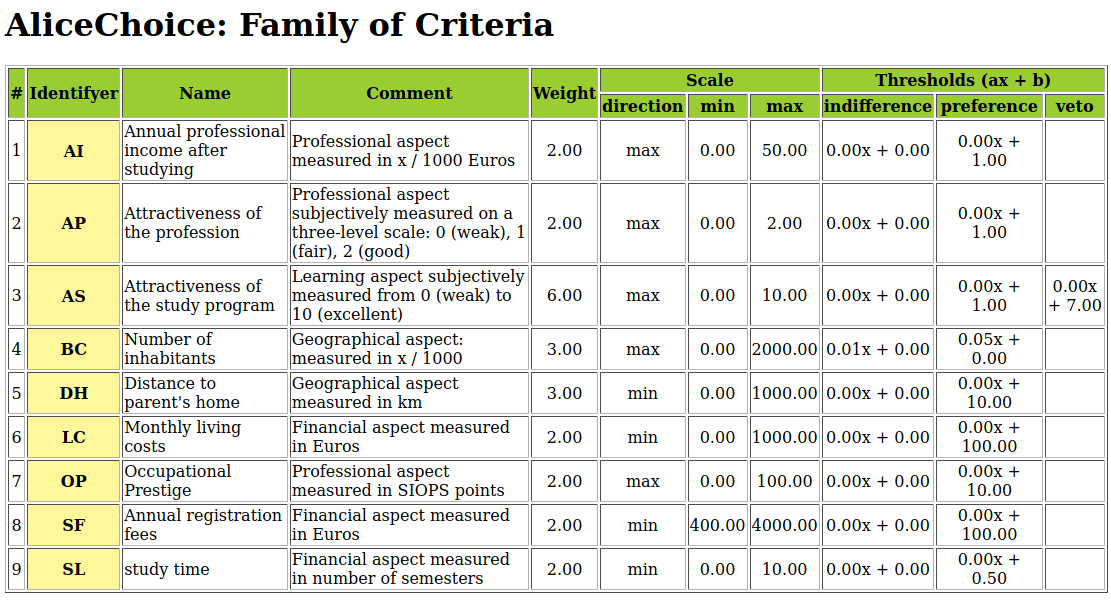
\includegraphics[width=\hsize]{Figures/12-2-aliceCriteria.png}
\caption{Alice's performance criteria}
\label{fig:12.2}       % Give a unique label
\end{figure}

It is worthwhile noticing in Fig.~\vref{fig:12.2} that, on her subjective attractiveness scale of the study programs (criterion \texttt{AS}), Alice considers a performance differences of 7 points to be \emph{considerable} and triggering, the case given, an outranking polarisation \citep{BIS-2013}. Notice also the proportional \emph{indifference} ($1\%$) and \emph{preference} ($5\%$) discrimination thresholds shown on criterion \texttt{BC} (number of inhabitants).

Alice is subjectively evaluating the \emph{Attractiveness} of the studies (criterion \texttt{AS}) on an ordinal scale from \emph{weak} ($0$) to \emph{excellent} ($10$). Similarly, she is subjectively evaluating the \emph{Attractiveness} of the respective professions (criterion \texttt{AP}) on a three level ordinal scale from \emph{weak} ($0$), \emph{fair} ($1$) to \emph{good} ($2$). Considering the \emph{Occupational Prestige} (criterion \texttt{OP}), she looked up the SIOPS \footnote{Standard International Occupational Prestige Scale \citep*{GAN-1996}.}. All the other evaluation data she found on the internet.

In the \emph{heatmap view} shown in Fig.~\vref{fig:12.3}, we may now consult Alice's performance gradings.
\begin{lstlisting}
>>> t.showHTMLPerformanceHeatmap(\
...       colorLevels=5,Correlations=True,ndigits=0)
\end{lstlisting}
\begin{figure}[ht]
%\sidecaption
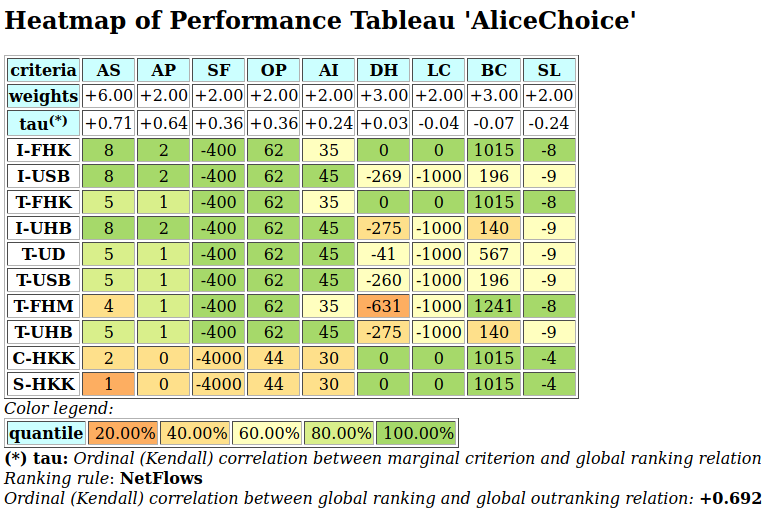
\includegraphics[width=\hsize]{Figures/12-3-aliceHeatmap.png}
\caption{Heatmap of Alice's performance tableau}
\label{fig:12.3}       % Give a unique label
\end{figure}

Her ten potential study programs are ordered with the \NetFlows ranking rule applied to the corresponding bipolar-valued outranking digraph (see Section~\vref{sec:8.3}). \emph{Graduate interpreter} studies in Köln (\texttt{I-FHK}) or Saarbrücken (\texttt{I-USB}), followed by \emph{Qualified Translator} studies in Köln (\texttt{T-FHK}) appear to be Alice's most preferred alternatives. The least attractive for her appear to be studies at the Chamber of Commerce of Köln (\texttt{C-HKK}, \texttt{S-HKK}). Notice by the way that evaluations on performance criteria to be \emph{minimized}, like \emph{Distance to Home} (criterion \texttt{DH}) or \emph{Study time} (criterion \texttt{SL}), are registered as \emph{negative} values, so that smaller measures are, in this case, preferred to larger ones.

It is finally interesting to observe in Fig.~\vref{fig:12.3} (third row) that the \emph{most significant} performance criteria, appear to be for Alice, on the one side, the \emph{Attractiveness} of the study program (criterion \texttt{AS}, tau = $+0.72$) followed by the \emph{Attractiveness} of the future profession (criterion \texttt{AP}, tau = $+0.62$). On the other side, \emph{Study times} (criterion \texttt{SL}, tau = $-0.24$), \emph{Big city} (criterion \texttt{BC}, tau = $-0.07$) as well as \emph{Monthly living costs} (criterion \texttt{LC}, tau = $-0.04$) appear to be \emph{not so significant} (see Chapter~\vref{sec:16}).

\section{Building a best choice recommendation}
\label{sec:12.3}

Let us now have a look at the resulting pairwise outranking situations.
\begin{lstlisting}[caption={Computing Alice's outranking digraph},label=list:12.2]
>>> from outrankingDigraphs import BipolarOutrankingDigraph
>>> dg = BipolarOutrankingDigraph(t) 
>>> dg
  *------- Object instance description ------*
   Instance class      : BipolarOutrankingDigraph
   Instance name       : rel_AliceChoice
   Actions             : 10
   Criteria            : 9
   Size                : 67
   Determinateness (%) : 73.91
   Valuation domain    : [-1.00;1.00]
>>> dg.computeSymmetryDegree(Comments=True)
  Symmetry degree of graph <rel_AliceChoice> : 0.49
\end{lstlisting}

From Alice's performance tableau we obtain in the digraph \texttt{dg}  67 positively validated pairwise outranking situations, supported by a $74\%$ majority of criteria significance (see Lines 9-10 in Listing~\vref{list:12.2}).

Due to the poorly discriminating performance evaluations, nearly half of these outranking situations (see Line 12) are \emph{symmetric} and reveal actually \emph{more or less indifference} situations between the potential study programs. This is well illustrated in the \emph{relation map} of the outranking digraph shown in Fig.~\vref{fig:12.4}.
\begin{figure}[ht]
%\sidecaption
\includegraphics[width=10cm]{Figures/12-4-aliceRelationmap.png}
\caption{\Copeland ranked outranking relation map}
\label{fig:12.4}       % Give a unique label
\end{figure}
\begin{lstlisting}
>>> dg.showHTMLRelationMap(\
...           tableTitle='Outranking relation map',\
...           rankingRule='Copeland')
\end{lstlisting}

We have mentioned that Alice considers a performance difference of $7$ points on the \emph{Attractiveness of studies} criterion \texttt{AS} to be considerable which triggers, the case given, a potential polarisation of the outranking characteristics. In Fig.~\vref{fig:12.4}, these polarisations appear in the last column and last row. We may inspect the occurrence of such polarisations with the \texttt{showPolarisations()} method. \index{showPolarisations@\texttt{showPolarisations()}}
\begin{lstlisting}[caption={Polarised outranking situations},label=list:12.3]
>>> dg.showPolarisations()
  *----  Negative polarisations ----*
   number of negative polarisations : 3 
    1: r(S-HKK >= I-FHK) = -0.17
     criterion: AS
     Considerable performance difference : -7.00
     Veto discrimination threshold       : -7.00
     Polarisation: r(S-HKK >= I-FHK) = -0.17 ==> -1.00
    2: r(S-HKK >= I-USB) = -0.17
     criterion: AS
     Considerable performance difference : -7.00
     Veto discrimination threshold       : -7.00
     Polarisation: r(S-HKK >= I-USB) = -0.17 ==> -1.00
    3: r(S-HKK >= I-UHB) = -0.17
     criterion: AS
     Considerable performance difference : -7.00
     Veto discrimination threshold       : -7.00
     Polarisation: r(S-HKK >= I-UHB) = -0.17 ==> -1.00
  *----  Positive polarisations ----*
   number of positive polarisations: 3 
    1: r(I-FHK >= S-HKK) = 0.83
     criterion: AS
     Considerable performance difference : 7.00
     Counter-veto threshold              : 7.00
     Polarisation: r(I-FHK >= S-HKK) = 0.83 ==> +1.00
    2: r(I-USB >= S-HKK) = 0.17
     criterion: AS
     Considerable performance difference : 7.00
     Counter-veto threshold              : 7.00
     Polarisation: r(I-USB >= S-HKK) = 0.17 ==> +1.00
    3: r(I-UHB >= S-HKK) = 0.17
     criterion: AS
     Considerable performance difference : 7.00
     Counter-veto threshold              : 7.00
     Polarisation: r(I-UHB >= S-HKK) = 0.17 ==> +1.00
\end{lstlisting}

In Listing~\vref{list:12.3}, we see that \emph{considerable} performance differences concerning the \emph{Attractiveness of the studies} (\texttt{AS} criterion) are indeed observed between the \emph{Specialised Secretary} study programm offered in Köln and the \emph{Graduate Interpreter} study programs offered in Köln, Saarbrücken and Heidelberg. They polarise, hence, three \emph{more or less invalid} outranking situations to \emph{certainly invalid} (Lines 8, 13, 18) and corresponding three \emph{more or less valid} converse outranking situations to \emph{certainly valid} ones (Lines 25, 30, 35). 

We may finally notice in the relation map, shown in Fig.~\vref{fig:12.4}, that the four best-ranked study programs, \texttt{I-FHK}, \texttt{I-USB}, \texttt{I-UHB} and \texttt{T-FHK},  are in fact \Condorcet winners (see Listing~\vref{list:12.4} Line 2), i.e. they are all four \emph{indifferent} one of the other \textbf{and} positively \emph{outranking} all other alternatives, a result confirmed in Listing~\vref{list:12.4} below by our \Rubis best choice recommendation \citep*{BIS-2008a}.
\begin{lstlisting}[caption={Alice's best choice recommendation},label=list:12.4]
>>> dg.computeCondorcetWinners()
  ['I-FHK', 'I-UHB', 'I-USB', 'T-FHK'] 
>>> dg.showBestChoiceRecommendation()
  Best choice recommendation(s) (BCR)
    (in decreasing order of determinateness)   
    Credibility domain: [-1.00,1.00]
   === >> potential best choice(s)
   choice                : ['I-FHK','I-UHB','I-USB','T-FHK']
     independence        : 0.17
     dominance           : 0.08
     absorbency          : -0.83
     covering (%)        : 62.50
     determinateness (%) : 68.75
     most credible action(s) = {'I-FHK': 0.75,'T-FHK': 0.17,
                                'I-USB': 0.17,'I-UHB': 0.17}
   === >> potential worst choice(s) 
   choice                : ['C-HKK', 'S-HKK']
     independence        : 0.50
     dominance           : -0.83
     absorbency          : 0.17
     covered (%)         : 100.00
     determinateness (%) : 58.33
     most credible action(s) = {'S-HKK': 0.17,'C-HKK': 0.17}
\end{lstlisting}

Most credible best choice among the four best-ranked study programs eventually becomes the \emph{Graduate Interpreter} study program at the Technical High School in Köln (see Line 14) supported by a $(0.75 + 1)/2.0 \,=\,87.5\% (18/24)$ majority of global criteria significance \footnote{See Section~\vref{sec:17.6} on solving \Berge kernel equation systems.}.

In the relation map, shown in Fig.~\vref{fig:12.4}, we see in the left lower corner that the \emph{asymmetric part} of the outranking relation, i.e. the corresponding \emph{strict} outranking relation, is actually \emph{transitive} (see Line 2 below). Hence, a \emph{graphviz} drawing of its \emph{skeleton}, oriented by the previous \emph{best}, respectively \emph{worst} choice, may well illustrate our \emph{best choice recommendation}.
\begin{lstlisting}[caption={Alice's strict best choice recommendation},label=list:12.5]
>>> dgcd = ~(-dg)
>>> dgcd.isTransitive()
    True
>>> dgcd.closeTransitive(Reverse=True,InSite=True)
>>> dgcd.exportGraphViz('aliceBestChoice',\
...                     bestChoice=['I-FHK'],\
...                     worstChoice=['S-HKK','C-HKK'])
  *---- exporting a dot file for GraphViz tools ---------*
   Exporting to aliceBestChoice.dot
   dot -Grankdir=BT -Tpng aliceBestChoice.dot -o aliceBestChoice.png
\end{lstlisting}
\begin{figure}[ht]
\sidecaption[t]
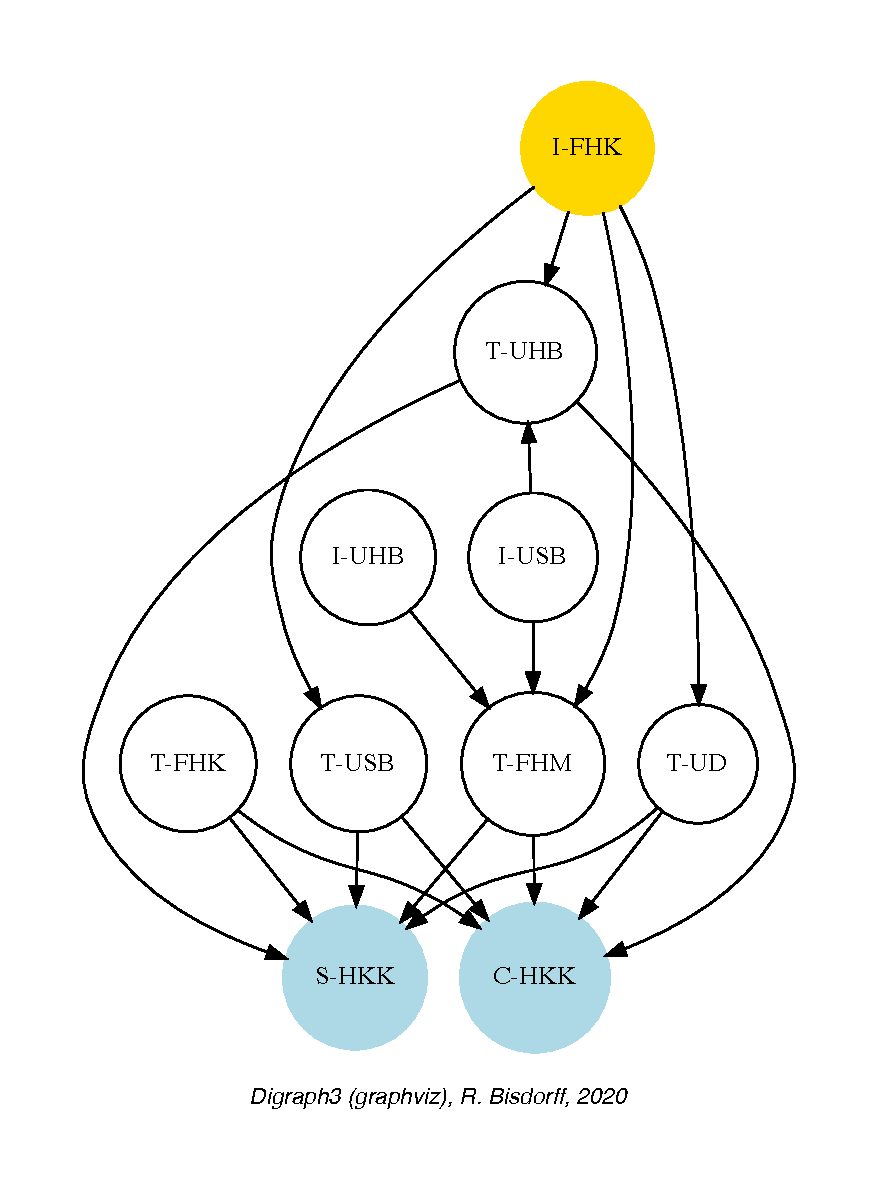
\includegraphics[width=7cm]{Figures/12-5-aliceBestChoice.pdf}
\caption{In Alice's best choice recommendation, we notice that the \emph{Graduate Interpreter} studies come first, followed by the \emph{Qualified Translator} studies. Last come the \emph{Chamber of Commerce}'s specialised studies. This confirms again the high significance that Alice attaches to the \emph{attractiveness} of her further studies and of her future profession (see criteria \texttt{AS} and \texttt{AP} in Fig.~\vref{fig:12.3})}
\label{fig:12.5}       % Give a unique label
\end{figure}

Let us now, for instance, check the pairwise outranking situations observed between the first and second-ranked alternative, i.e. \emph{Garduate Interpreter} studies in Köln versus \emph{Graduate Interpreter} studies in Saabrücken (see \texttt{I-FHK} and \texttt{I-USB} in Fig.~\vref{fig:12.3}).
\begin{lstlisting}
>>> dg.showHTMLPairwiseOutrankings('I-FHK','I-USB')
\end{lstlisting}
\begin{figure}[ht]
\sidecaption[t]
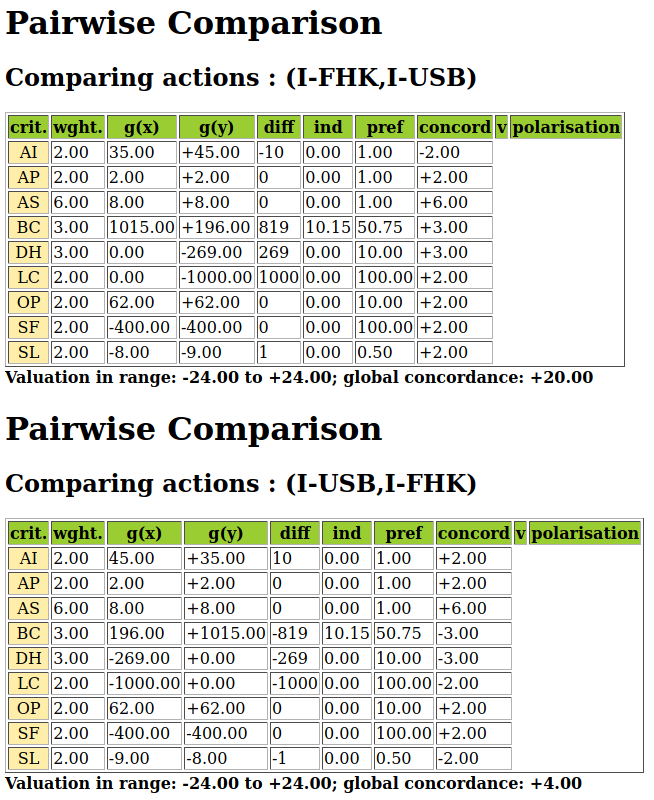
\includegraphics[width=7cm]{Figures/12-6-pairwiseComparison.png}
\caption{Comparing the first and second best-ranked study programs. The Köln alternative is performing \emph{at least as well as} the Saarbrücken alternative on all the performance criteria, except the \emph{Annual income} (of significance $2/24$). Conversely, the Saarbrücken alternative is clearly \emph{outperformed} from the geographical ($0/6$) as well as from the financial perspective ($2/6$)}
\label{fig:12.6}       % Give a unique label
\end{figure}
%\clearpage

In a similar way, one may finally compute a \emph{weak ranking} of all the potential study programs with the help of the \texttt{RankingByChoosingDigraph} constructor\index{RankingByChoosingDigraph@\texttt{RankingByChoosingDigraph} class}, that computes a bipolar ranking by conjointly \emph{best-choosing} and \emph{last-rejecting} \citep{BIS-1999}.
\begin{lstlisting}[caption={Weakly ranking by bipolar best-choosing and last-rejecting},label=list:12.6]
>>> from transitiveDigraphs import\
...               RankingByChoosingDigraph
>>> rbc = RankingByChoosingDigraph(dg)
>>> rbc.showRankingByChoosing()
    Ranking by Choosing and Rejecting
     1st ranked ['I-FHK'] 
       2nd ranked ['I-USB']
	 3rd ranked ['I-UHB']
	   4th ranked ['T-FHK']
	     5th ranked ['T-UD']
	     5th last ranked ['T-UD']
	   4th last ranked ['T-UHB', 'T-USB']
	 3rd last ranked ['T-FHM']
       2nd last ranked ['C-HKK']
     1st last ranked ['S-HKK']
\end{lstlisting}

In Listing~\vref{list:12.6}, we find confirmed that the \emph{Interpreter} studies appear all preferrred to the \emph{Translator} studies. Furthermore, the \emph{Interpreter} studies in Saarbrücken appear preferred to the same studies in Heidelberg. The Köln alternative is apparently the preferred one of all the \emph{Translater} studies. And, the \emph{Foreign Correspondent} and the \emph{Specialised Secretary} studies appear second-last and last ranked.

Yet, how \emph{robust} are our findings with respect to potential settings of the decision objectives' importance and the performance criteria significance?
		
\section{Robustness analysis}
\label{sec:12.4}

Alice considers her four decision objectives as being \emph{more or less} equally important. Here we have, however, allocated \emph{strictly equal} importance weights with \emph{strictly equi-significant} criteria per objective. How robust is our previous best choice recommendation when, now, we would consider the importance of the objectives and, hence, the significance of the respective performance criteria to be \emph{more or less uncertain}?

To answer this question, we will consider the respective criteria significance weights $w_j$ for $j=1,...,9$ to be \emph{triangular random variables} in the range 0 to $2w_j$ with mode = $w_j$. We may compute a corresponding $90\%$-\emph{confident} outranking digraph with the help of the \texttt{ConfidentBipolarOutrankingDigraph} constructor\index{ConfidentBipolarOutrankingDigraph@\texttt{ConfidentBipolarOutrankingDigraph} class} (see Chapter~\vref{sec:18}).
\begin{lstlisting}[caption={Computing the 90\% confident outranking digraph},label=list:12.7]
>>> from outrankingDigraphs import\
...         ConfidentBipolarOutrankingDigraph
>>> cdg = ConfidentBipolarOutrankingDigraph(t,\
...         distribution='triangular',confidence=90.0)
>>> cdg
  *------- Object instance description ------*
    Instance class       : ConfidentBipolarOutrankingDigraph
    Instance name        : rel_AliceChoice_CLT
    Actions              : 10
    Criteria             : 9
    Size                 : 44
    Valuation domain     : [-1.00;1.00]
    Uncertainty model    : triangular(a=0,b=2w) 
    Likelihood domain    : [-1.0;+1.0] 
    Confidence level     : 90.0% 
    Confident majority   : 14/24 (58.3%) 
    Determinateness (%)  : 68.19
\end{lstlisting}

Of the original 67 valid outranking situations, we retain 44 outranking situations as being $90\%$-confident (see Listing~\vref{list:12.7} Line 11). The corresponding $90\%$-confident \emph{qualified majority} of criteria significance amounts to $14/24 = 58.3\%$ (Line 16).  

Concerning now a $90\%$-confident best choice recommendation, we are lucky. 
\begin{lstlisting}[caption={Computing the $90\%$-confident best choice recommendation.},label=list:12.8]
>>> cdg.computeCondorcetWinners()
  ['I-FHK']
>>> cdg.showBestChoiceRecommendation()
  ***********************
  Best choice recommendation(s) (BCR)
   (in decreasing order of determinateness)   
   Credibility domain: [-1.00,1.00]
  === >> potential best choice(s)
   choice              : ['I-FHK','I-UHB','I-USB',
                          'T-FHK','T-FHM']
      independence        : 0.00
      dominance           : 0.42
      absorbency          : 0.00
      covering (%)        : 20.00
      determinateness (%) : 61.25
   - most credible action(s) = { 'I-FHK': 0.75, }
\end{lstlisting}

The \emph{Graduate Interpreter} studies in Köln remain indeed a 90\%-confident \Condorcet winner (see Fig.~\vref{fig:12.7} Line 2). Hence, the same study program also remains our 90\%-confident most credible best choice supported by a continual $18/24 (87.5\%)$ majority of the global criteria significance (see Lines 9-10 and 16 in Listing~\vref{list:12.8}).

When previously comparing the two best-ranked study programs (see Fig.~\vref{fig:12.6}), we have observed that \texttt{I-FHK} actually positively outranks \texttt{I-USB} on all four decision objectives. When admitting equi-significant criteria significances per objective, this outranking situation is hence valid independently of the importance weights Alice may allocate to each of her decision objectives. 

The \texttt{UnOpposedBipolarOutrankingDigraph} class constructor computes these \emph{unopposed} outranking situations (see Section~\vref{sec:19.5}).
\begin{lstlisting}[caption={Computing the unopposed outranking situations},label=list:12.9]
>>> from outrankingDigraphs import\
...                     UnOpposedBipolarOutrankingDigraph
>>> uop = UnOpposedBipolarOutrankingDigraph(t)
>>> uop
  *------- Object instance description ------*
   Instance class       : UnOpposedBipolarOutrankingDigraph
   Instance name        : AliceChoice_unopposed_outrankings
   Actions              : 10
   Criteria             : 9
   Size                 : 28
   Oppositeness (%)     : 58.21
   Determinateness (%)  : 62.94
   Valuation domain     : [-1.00;1.00]
>>> uop.isTransitive()
  True
\end{lstlisting}

We keep 28 out the 67 standard outranking situations, which leads to an \emph{oppositeness degree} of $(1.0 - 28/67) = 58.21\%$ (see Lines 10-11 in Listing~\vref{list:12.9}). Remarkable furthermore is that this unopposed outranking digraph \texttt{uop} is actually \emph{transitive}, i.e. modelling a \emph{partial ranking} of the study programs (Lines 14-15).

We may hence make use of the \texttt{exportGraphViz()} method of the \texttt{Transi\-tiveDigraph} class\index{TransitiveDigraph@\texttt{TransitiveDigraph} class} for drawing the corresponding partial ranking.
\begin{lstlisting}
>>> from transitiveDigraphs import TransitiveDigraph
>>> TransitiveDigraph.exportGraphViz(uop,\
...           fileName='choiceUnopposed')
  *---- exporting a dot file for GraphViz tools ---------*
   Exporting to choiceUnopposed.dot
   dot -Grankdir=TB -Tpng choiceUnopposed.dot -o choiceUnopposed.png
\end{lstlisting}
\begin{figure}[ht]
\sidecaption[t]
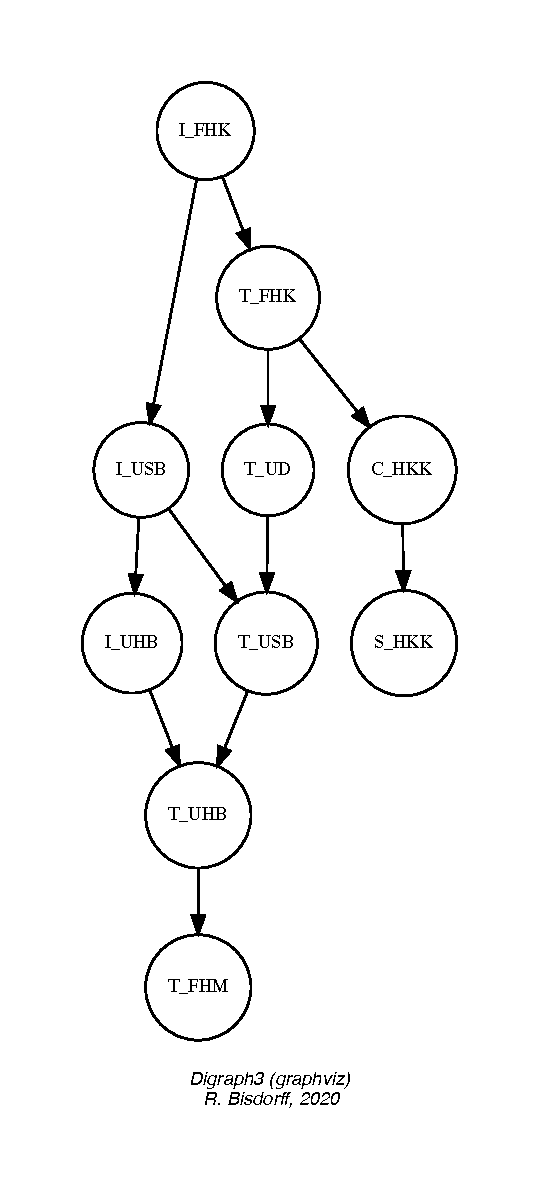
\includegraphics[width=6cm]{Figures/12-7-choiceUnopposed.pdf}
\caption{Unopposed partial ranking of the potential study programs. Again, when \emph{equi-signficant} performance criteria are assumed per decision objective, we observe in the Figure here that $I-FHK$ remains the stable best choice, \emph{independently} of the actual importance weights that Alice may wish to allocate to her four decision objectives}
\label{fig:12.7}       % Give a unique label
\end{figure}
%\clearpage

In view of her performance tableau shown in Fig.~\vref{fig:12.3}, \emph{Graduate Interpreter} studies at the Technical High School Köln, thus, represent definitely \textbf{Alice's very best choice}.

For further reading about the \Rubis \emph{Best Choice} methodology, one may consult in \citet{BIS-2015bestPoster} the study of a \emph{real decision aid case} about choosing a best poster in a scientific conference.
 
%%%%%%% The chapter bibliography
%\normallatexbib
\clearpage
%\phantomsection
%\addcontentsline{toc}{section}{Chapter Bibliography}
\bibliographystyle{spbasic}
%\typeout{}
\bibliography{03-backMatters/reference}
%\input{02-mainMatters/12-chapterAliceChoice.bbl}
\bibliographystyle{spbasic}
\bibliography{03-backMatters/reference}
